\documentclass[twocolumn,aps,prd,floatfix,preprintnumbers,a4paper,nofootinbib,
superscriptaddress,10pt]{revtex4-1}

\usepackage{epsfig}
\usepackage{graphics}
\usepackage{graphicx}
\usepackage{amsmath,amssymb,mathtools}
\usepackage{amsfonts}
\usepackage{bm,soul}
\usepackage[usenames,dvipsnames]{color}
\usepackage{amssymb}
\usepackage{url}
\usepackage{psfrag}
\usepackage{times}
\usepackage[varg]{txfonts}
\usepackage[colorlinks, pdfborder={0 0 0}]{hyperref}
\usepackage{lineno}
\usepackage{verbatim}
\definecolor{LinkColor}{rgb}{0.75, 0, 0}
\definecolor{CiteColor}{rgb}{0.75, 0, 0}
\definecolor{UrlColor}{rgb}{0, 0, 0.75}
\hypersetup{linkcolor=LinkColor}
\hypersetup{citecolor=CiteColor}
\hypersetup{urlcolor=UrlColor}
\usepackage[utf8]{inputenc}
\usepackage{ulem}
\normalem
\hoffset -0.17in
\voffset 0.3in
\textheight 10in

\usepackage{algorithm}
\usepackage{algpseudocode} % in place of algorithmic. Conflicts with revtex4 unless [H] option passed
\usepackage{setspace} % for pleasent spacing in algorithm

%%%%%%%%%%%%%%%%%%%%%%%%%%%%%%%% Useful Definitions %%%%%%%%%%%%%%%%%%%%%%%%%%%%%%%%%%%%%%%%%

% definitions


\usepackage{inputenc}
\usepackage{pgfplots}
\usepackage{tikz}
\usetikzlibrary{shapes,arrows}
\usetikzlibrary{positioning}
\usetikzlibrary{backgrounds}

\def\singleline{
	\begin{center}
	\line(1,0){250}
	\end{center}
}

\newenvironment{aside}
    {\begin{addmargin}[1em]{2em}% 2em left, 1em right
\begin{center} \noindent\rule{0.65\paperwidth}{0.4pt} \end{center}
    }
    {
    \begin{center} \noindent\rule{0.65\paperwidth}{0.4pt} \end{center}
\end{addmargin}
    }

% CUSTOM COMMANDS
\newcommand\xquote[1]{``#1"}
\newcommand\psinr[2]{$\psi_{{#1}{#2}}^{NR}$}
% \newcommand\red[1]{{\color{red} #1}}
\newcommand\red[1]{{\color[rgb]{0.75,0.0,0.0} #1}}
\newcommand\green[1]{{\color[rgb]{0.0,0.60,0.08} #1}}
\newcommand\blue[1]{{\color[rgb]{0,0.20,0.65} #1}}
\newcommand\cyan[1]{{\color[HTML]{00c3ff} #1}}
\newcommand\bluey[1]{{\color[rgb]{0.11,0.20,0.4} #1}}
\newcommand\gray[1]{{\color[rgb]{0.7,0.70,0.7} #1}}
\newcommand\grey[1]{{\color[rgb]{0.7,0.70,0.7} #1}}
\newcommand\white[1]{{\color[rgb]{1,1,1} #1}}
\newcommand\darkgray[1]{{\color[rgb]{0.3,0.30,0.3} #1}}
\newcommand\orange[1]{{\color[rgb]{.86,0.24,0.08} #1}}
\newcommand\purple[1]{{\color[rgb]{0.45,0.10,0.45} #1}}
\newcommand\note[1]{\colorbox[rgb]{0.85,0.94,1}{\textcolor{black}{\textsc{\textsf{#1}}}}}

%
\newcommand*{\figfactor}{0.495}

% Math symbols
% ###################################### %
%\def\mh{{\hat{h}}} % model  for strain
\def\m#1{{\hat{#1}}} % model  for strain
\def\ma#1{{\hat{#1}_{\bm{a}}}} % model  for strain
\newcommand{\var}[1]{\mathcal{{#1}}}
\newcommand{\mlam}{{\bm{\lambda}}}
\newcommand{\lam}{{\lambda}}
\newcommand{\mLam}{{\bm{\Lambda}}}
\newcommand{\bigo}[1]{{\cal O}({#1})}
\newcommand{\braket}[2]{ {\langle {#1} | {#2} \rangle} }
% ###################################### %

% ###################################### %
\definecolor{lightblue}{rgb}{.82,.88,0.95}
\definecolor{lightred}{rgb}{0.95,.86,0.86}
\definecolor{yellow}{rgb}{0.95,0.95,0.86}
\definecolor{green}{rgb}{.90,1,0.95}
\definecolor{lightpurple}{rgb}{.95,0.85,0.95}
% ###################################### %

\tikzset{
    vertex/.style = {
        circle,
        fill            = black,
        outer sep = 2pt,
        inner sep = 1pt,
    }
}


% CUSTOM DEFINITIONS
% ***************************************** %
\def\prd{Phys.Rev.D}
% ***************************************** %
\def\gt{Georgia Tech}
% ***************************************** %
\def\tk{Teukolsky}
% ***************************************** %
\def\mp{multipole}
% ***************************************** %
\def\ee{Einstein's equations}
% ***************************************** %
\def\toolkit#1{NRDA--Toolkit{#1}}
% \def\toolkit#1{Data Analysis Toolkit{#1}}
% ***************************************** %
\def\wf#1{waveform#1}
% ***************************************** %
\def\grad#1{gravitational radiation#1}
% ***************************************** %
\def\gr#1{General Relativity#1}
% ***************************************** %
\def\gwa#1{Gravitational Wave Astrophysics#1}
% ***************************************** %
\def\gwf#1{gravitational waveform#1}
% ***************************************** %
\def\gw#1{gravitational wave#1}
% ***************************************** %
\def\gwa#1{\gw{} astronomy#1}
% ***************************************** %
\def\nht#1{No-Hair Theorem#1}
% ***************************************** %
\def\rm#1{\mathrm{#1}}
% ***************************************** %


% Referencing
% ***************************************** %
\def\prt#1{Part~(\ref{#1})}
% ***************************************** %
\def\ap#1{Appendix~(\ref{#1})}
% ***************************************** %
\def\ch#1{Chapter~(\ref{#1})}
% ***************************************** %
\def\cch#1{Chapter~\ref{#1}}
% ***************************************** %
\newcommand{\chs}[2]{Chapters~(\ref{#1}-\ref{#2})}
% ***************************************** %
\newcommand{\cchs}[2]{Chapters~\ref{#1}-\ref{#2}}
% ***************************************** %
\def\sec#1{Section~(\ref{#1})}
% ***************************************** %
\def\csec#1{Section~\ref{#1}}
% ***************************************** %
\def\tk#1{Teukolsky#1}
% ***************************************** %
\newcommand{\secs}[2]{Sections~(\ref{#1}-\ref{#2})}
% ***************************************** %
\def\fig#1{Fig.~\ref{#1}} % NOTE that PRL requires that Fig. be used rather
% than figure
% \def\fig#1{\hyperref[#1]{Figure~\ref{#1}}}
% ***************************************** %
\def\cfig#1{Fig.~\ref{#1}}
% \def\cfig#1{Figure~\ref{#1}}
% ***************************************** %
\newcommand{\figs}[2]{Figures~(\ref{#1}-\ref{#2})}
% ***************************************** %
\def\eqn#1{Eqn.~(\ref{#1})}
% \def\eqn#1{Equation~(\ref{#1})}
% ***************************************** %
\def\ceqn#1{Eqn.~\ref{#1}}
% \def\ceqn#1{Equation~\ref{#1}}
% ***************************************** %
\newcommand{\eqns}[2]{Equations~(\ref{#1})--(\ref{#2})}
% ***************************************** %
\newcommand{\ceqns}[2]{Equations~\ref{#1}--\ref{#2}}
% ***************************************** %
\def\tbl#1{Table~(\ref{#1})}
% ***************************************** %
\def\ctbl#1{Table~\ref{#1}}
% ***************************************** %


% ***************************************** %
\def\da#1{data analysis#1}
% ***************************************** %
\def\imr#1{inspiral, merger and ringdown#1
  (IMR#1)\gdef\imr{IMR}}
% ***************************************** %
\def\lal#1{LIGO Analysis Library#1
  (LAL#1)\gdef\lal{LAL}}
% ***************************************** %
\def\nrda#1{\nr{} Data Analysis#1
  (NRDA#1)\gdef\nrda{NRDA}}
% ***************************************** %
\def\tt#1{\textit{transverse--traceless}#1
  (TT#1)\gdef\tt{TT}}
% ***************************************** %
\def\et#1{Einstein Telescope#1
  (ET#1)\gdef\et{ET}}
% ***************************************** %
\def\ego#1{European Gravitational Observatory#1
  (EGO#1)\gdef\ego{EGO}}
% ***************************************** %
\def\elisa#1{Evolved Laser Interferometer Space Antenna#1
  (eLISA#1)\gdef\elisa{eLISA}}
% ***************************************** %
\def\ligo#1{Laser Interferometer Gravitational Wave Observatory#1
  (LIGO#1)\gdef\ligo{LIGO}}
% \def\ligo#1{LIGO#1}
% ***************************************** %
\def\virgo#1{Virgo#1}
% ***************************************** %
\def\aligo#1{Advanced LIGO#1
  (aLIGO#1)\gdef\aligo{aLIGO}}
% ***************************************** %
\def\snr#1{signal-to-noise ratio#1
  (SNR#1)\gdef\snr{SNR}}
% ***************************************** %
\def\psd#1{power spectral density#1
  (PSD#1)\gdef\psd{PSD}}
% ***************************************** %
\def\rom#1{reduced order model#1
  (ROM#1)\gdef\rom{ROM}}
% ***************************************** %
\def\gatech#1{Georgia Institute of Technology#1
  (GaTech#1)\gdef\gatech{GaTech}}
% ***************************************** %
\def\ffi#1{Fixed-Frequrncy Integration#1
  (FFI#1)\gdef\ffi{FFI}}
% ***************************************** %
\def\sxs#1{Simulating Extreme Spacetimes#1
  (SXS#1)\gdef\sxs{SXS}}
% ***************************************** %
\def\bam#1{Bifunctional Adaptive Mesh#1
  (BAM#1)\gdef\bam{BAM}}
% ***************************************** %
\def\adm#1{Arnowitt-Deser-Misner
	(ADM#1)\gdef\adm{ADM}}
%
\def\frmse#1{Fractional Root-Mean Square Error
	(FRMSE)\gdef\frmse{FRMSE}}


% ***************************************** %
\def\bh#1{black hole#1
 (BH#1)\gdef\bh{BH}}
% \def\bh#1{black hole#1}
% ***************************************** %
%\def\bbh#1{binary black hole#1
%  (BBH#1)\gdef\bbh{BBH}}
\def\bbh#1{binary \bh{}#1}
% ***************************************** %
\def\bhb#1{\bh{} binary#1}
% ***************************************** %


% ***************************************** %
\def\qnm#1{Quasi-Normal Mode#1
  (QNM#1)\gdef\qnm{QNM}}
% ***************************************** %
\def\eob#1{Effective One Body#1
  (EOB#1)\gdef\eob{EOB}}
% ***************************************** %
\def\gw#1{gravitational-wave#1}
\def\gw#1{Gravitational wave#1
 (GW#1)\gdef\gw{GW}}
% ***************************************** %
\def\gwa#1{gravitational wave astronomy#1}
% ***************************************** %
\def\spa#1{stationary phase approximation#1
 (SPA#1)\gdef\spa{SPA}}
% ***************************************** %
\def\pn#1{Post-Newtonian#1
	(PN#1)\gdef\pn{PN}}
% ***************************************** %
\def\pnl#1{post-Newtonian-like#1
  (PN-like#1)\gdef\pnl{PN-like}}
% ***************************************** %
% \def\nr{Numerical Relativity}
\def\NR{{\text{NR}}}
\def\nr{Numerical Relativity
 (NR)\gdef\nr{NR}}
% ***************************************** %
\def\pt{perturbation theory}
% ***************************************** %
\def\GOLS#1{\textit{greedy ordinary least-squares}#1}
% ***************************************** %
\def\rd{ringdown}
% ***************************************** %
% \def\imr{inspiral, merger and \rd{}}
% ***************************************** %
\def\cbc#1{compact object coalescence#1}
% ***************************************** %
\def\bbc#1{binary black hole coalescence#1}
%\def\bbc#1{binary black hole coalescence#1
%  (BBC#1)\gdef\bbc{BBC}}
% ***************************************** %
\def\pc#1{principle component#1}
% ***************************************** %
\def\pca#1{principle component analysis#1
  (PCA#1)\gdef\pca{PCA}}
% ***************************************** %
\def\svd#1{Singular Value Decomposition#1
  (SVD#1)\gdef\svd{SVD}}
% ***************************************** %
\def\gs#1{Gram-Schmidt#1}
% ***************************************** %
% ***************************************** %
\newcommand*{\factor}{0.95} % for figure scale
\newcommand*{\rscale}{1.3}
% ***************************************** %

% ******************************************************* %
\def\study{work} %
% ******************************************************* %

\newcommand{\osum}{\operatornamewithlimits{
\hspace{-2pt}{\bigcup\hspace{-9.5pt}\circ}
}}

% commutative multiplication
\newcommand{\ox}{\operatornamewithlimits{
{\circ\hspace{-3.7pt}\cdot}
}}

% non-commutative multiplication
\newcommand{\cc}{ \circledcirc }

% general subtraction
\newcommand{\om}{ \mathrel{\raisebox{1pt}{$\scriptscriptstyle\circleddash$}} }






\newcommand{\hlgreen}[1]{\sethlcolor{green}\hl{#1}{\sethlcolor{yellow}}}
\newcommand{\hlyellow}[1]{\sethlcolor{yellow}\hl{#1}{\sethlcolor{yellow}}}
\newcommand{\hlblue}[1]{\sethlcolor{lightblue}\hl{#1}{\sethlcolor{yellow}}}
\newcommand{\hlred}[1]{\sethlcolor{lightred}\hl{#1}{\sethlcolor{yellow}}}
\newcommand{\hlpurple}[1]{\sethlcolor{lightpurple}\hl{#1}{\sethlcolor{yellow}}}

\newcommand{\hlbackground}[1]{\sethlcolor{green}\hl{#1}{\sethlcolor{yellow}}}
\newcommand{\hlproblem}[1]{\sethlcolor{yellow}\hl{#1}{\sethlcolor{yellow}}}
\newcommand{\hlmethods}[1]{\sethlcolor{lightblue}\hl{#1}{\sethlcolor{yellow}}}
\newcommand{\hlresults}[1]{\sethlcolor{lightred}\hl{#1}{\sethlcolor{yellow}}}
\newcommand{\hldiscussion}[1]{\sethlcolor{lightpurple}\hl{#1}{\sethlcolor{yellow}}}


% Richard's stuff

\newcommand\aap{\&A}
\newcommand\apss{APSS}
\newcommand\aaps{AAPS}
\newcommand\apjs{ApJ S}
\newcommand\aj{AJ}
\newcommand\apjl{ApJL}
\newcommand\mnras{MNRAS}
\newcommand\pasp{PASP}
\newcommand\araa{ARAA}
\newcommand\physrep{Phys. Rep.}

\newcommand\nrRequest{\textbf{NR INPUT?}}
\newcommand\richardBugFix{\textbf{\color{red}Richard will bugfix}}
\newcommand\editremark[1]{ {\color{red} #1}}
\newcommand\newtext[1]{{\bf #1}}
\newcommand\recentlychanged[1]{{\bf #1}}
\newcommand\hidetosubmit[1]{}
%
\newcommand\optional[1]{}
\newcommand\ForInternalReference[1]{}
\newcommand\embrace[1]{{[#1]}}
\newcommand\unit[1]{\, {\rm #1}}
\newcommand\mc{ {{\cal M}_c}}
\newcommand\Dho{ {D_{\rm H}^{(0)}}}
\newcommand\Dh{ {D_{\rm H}}}
\newcommand\Deff{{D_{\rm eff}}}  %
\newcommand\Dv{{D_{\rm v}}}      %
\newcommand\Dc{{D_c}}            %
\newcommand\Y[1]{Y^{(#1)}}


\newcommand\avL{\left< {\cal L}_{(a} {\cal L}_{b)} \right>}
\newcommand\WeylScalar{{\psi_4}}
\newcommand\WeylScalarFourier{{\tilde{\psi}_4{}}}
\newcommand\FourierWeylScalar{{\tilde{\psi}_4}}
\newcommand\WeylScalarCorot{R^{-1}{\psi_4}}

\newcommand\qmstate[1]{\left|#1\right>}
\newcommand\qmstateKet[1]{\left<#1\right|}
\newcommand\qmstateproduct[2]{\left<#1|#2\right>}
\newcommand\qmoperatorelement[3]{\left<#1\left|#2\right|#3\right>}
\newcommand\qmoperator[1]{{\bf #1}}
\newcommand\myvector[1]{{\mathbf{#1}}}
\newcommand\chip{{\boldsymbol{\chi}_+}}
\newcommand\chim{{\boldsymbol{\chi}_-}}

\newcommand\nSimulationsTotal{224}   %
\newcommand\nSimulationsNonprecessing{62}  %
\newcommand\ReferenceMassLow{100}      %
\newcommand\ReferenceMassMiddle{300}   %
\newcommand\ReferenceMassHigh{1000}   %


\newcommand\abbrvPSgrbs{PS-GRB}
\newcommand\abbrvCBC{CBC}

\def\check#1{\red{#1}}
\def\remove#1{\hlred{#1}}
\newcommand{\cw}{\tilde{\omega}}
\newcommand{\CW}{\tilde{\Omega}}
\newcommand{\CWr}{{\Omega}^{\mathrm{r}}}
\newcommand{\CWc}{{\Omega}^{\mathrm{c}}}
\newcommand{\SC}{\mathcal{K}}
\newcommand{\CC}{\mathcal{C}}
\newcommand{\SCr}{\mathcal{K}^{\mathrm{r}}}
\newcommand{\SCc}{\mathcal{K}^{\mathrm{c}}}
\newcommand{\lalapprox}{\texttt{MMRDNS}}
\def\jf{j_f}
\def\mf{M_f}
\newcommand{\LL}{\bar{l}}
\newcommand{\MM}{\bar{m}}
\def\lmn{_{\ell m n}}
\def\LM{_{\bar{\ell} \bar{m}}}
\def\LMlmn{_{\bar{\ell} \bar{m} \ell m n}}
\def\gmvp#1{greedy-multivariate-polynomial#1
  (\texttt{GMVP}#1)\gdef\gmvp{\texttt{GMVP}}}
\def\gmvr#1{greedy-multivariate-rational#1
  (\texttt{GMVR}#1)\gdef\gmvr{\texttt{GMVR}}}

\newcommand{\lmtitle}[2]{\vspace{-0.80cm} \begin{center} \noindent\rule{0.35\paperwidth}{0.3pt} \end{center} \vspace{-0.3cm}}

% Numbers that may change from time to time
\def\CwFitCalibrationRegion{\red{0.995} }
\def\NumCalibrationPointsPlotted{\red{21} }
\def\NumCalibrationPoints{\red{61} }

\newcommand{\Cardiff}{School of Physics and Astronomy, Cardiff University, Queens Buildings, Cardiff, CF24 3AA, United Kingdom}

%%%%%%%%%%%%%%%%%%%%%%%%%%%%%%%%%%%%%%%%%%%%%%%%%%%%%%%%%%%%%%%%%%%%%%%%%%%%%%%%%%%%%%%%%%%%%

\begin{document}

%%%%%%%%%%%%%%%%%%%%%%%%%%%%%%%%%%%%%% Title page %%%%%%%%%%%%%%%%%%%%%%%%%%%%%%%%%%%%%%%%%%%

\title{On modeling for Kerr black holes: Basis learning, QNM frequencies, and spherical-spheroidal mixing coefficients }

\author{L. London}
\affiliation{\Cardiff}
\author{E. Fauchon-Jones}
\affiliation{\Cardiff}

%%%%%%%%%%%%%%%%%%%%%%%%%%%%%%%%%%%%% Abstract %%%%%%%%%%%%%%%%%%%%%%%%%%%%%%%%%%%%%%%%
\begin{abstract}
	%
	The ongoing direct detection of gravitational wave signals is aided by representative models of theoretical predictions. In particular, the process of model based detection, and subsequent comparison of signals the general relativity's predictions are aided by the modeling of information related to perturbed Kerr black holes. Here, we summarize recent methods and models for the analytically understood gravitational wave spectra (quasi-normal mode frequencies), and harmonic structure of Kerr black holes (mixing coefficients between spherical and spheroidal harmonics). Towards the construction of these models, two algorithms, GMVP and GMVR, for the automated polynomial and rational modeling of general dimensional complex scalars are presented. GMVR is a quasi-linear numerical method for interpolating rational functions. It therefore represents a solution to the problem of Runge's phenomenon.
	%
\end{abstract}
%%%%%%%%%%%%%%%%%%%%%%%%%%%%%%%%%%%%%%%%%%%%%%%%%%%%%%%%%%%%%%%%%%%%%%%%%%%%%%%%%%%%%%%%

%%%%%%%%%%%%%%%%%%%%%%%%%%%%%%%%%%%% Preprint numbers %%%%%%%%%%%%%%%%%%%%%%%%%%%%%%%%%%
%\preprint{LIGO-P1500185-v10}
\date{\today}
%%%%%%%%%%%%%%%%%%%%%%%%%%%%%%%%%%%%%%%%%%%%%%%%%%%%%%%%%%%%%%%%%%%%%%%%%%%%%%%%%%%%%%%%

\maketitle

% \begin{itemize}
% 	\item BH detections happen, and use fits at various levels
% 	\item Fits for Kerr are important for modeling and testing GR, they are fast to eval comapred to formal calculations which has data analysis implications
% 	\item Many fits have been done for perturbative Kerr parameters: QNM frequencies most prominently.
% 	\item The problem/motivation:
% 		\begin{itemize}
% 			\item 1. There are many fits, and we would like to provide a reference for many of them, including key methods
% 			\item 2. Methods for fits: basis learning
% 			\item 3. (results) Summarize "simple fits": QNM frequencies and decay times, enforcing zero damping
% 			\item 4. (results) Summarize more general fits: mixing coefficients
% 		\end{itemize}
% 	\item (discussion) We have presented ...
% \end{itemize}

\section{Introduction}
%
In the coming years, expectations for frequent \gw{} detections of increasing \snr{} are high.
%
Concurrent with \virgo{}, the \aligo{} detectors will enter their third observing run in \check{late 2018}.
%
At this time, \bbh{} detections are expected at a rate of \check{X} per month.
%
In this context, signal detection and subsequent inference of physical parameters hinges upon efficient models for source properties and dynamics.
%
Most prominently, there is ongoing interest in signal models for \bbh{} \imr{}.
%
As the merger of isolated \bh{s} is expected to result in a perturbed Kerr \bh{}, there is related interest in having computationally efficient models for perturbative parameters, namely those that enable evaluation of the related \rd{} radiation.
%
\par In particular, a perturbed Kerr \bh{} (e.g. resulting from \bbh{} merger) will have \gw{} radiation that rings down with characteristic frequencies,
%
$%\begin{align}
	\cw\lmn = \omega\lmn + i/\tau\lmn
$%\end{align}
.
%
These discrete frequencies have associated radial and spatial functions which are \textit{spheroidal} harmonic in nature.
%
These frequencies and harmonic functions are the so-called \qnm{s}.
%
They are the eigen-solutions of the source free linearized \ee{} (i.e. \tk{'s} equations) for a perturbed \bh{} with final mass, $\mf$, and dimensionless final spin, $\jf$.
%
The well known and effective completeness of these solutions allows \grad{} from generic perturbations to be well approximated by a spectral (multipolar) sum which combines the complex \qnm{} amplitude, $A\lmn$, with the spin weight -2 spheroidal harmonics, $_{-2}S\lmn$.
%
\begin{align}
	%
	\label{hrd}
	%
	h &= h_{+} - i \, h_{\times}
	  \\ \nonumber
	  &= \frac{1}{r} \sum\lmn A\lmn \; e^{i\,\cw\lmn t} \; _{-2}S\lmn( \jf \cw\lmn,\theta,\phi)
		\\ \nonumber
		&= \frac{1}{r} \sum\LM h\LM(t) \; _{-2}Y\LM(\theta,\phi) \;  .
	%
\end{align}
%
\par In the first and second lines of \eqn{hrd}, we relate the observable \gw{} polarizations, $h_+$ and $h_\times$, with the analytically understood morphology of the time domain waveform.
%
Here, the labels $\ell$ and $m$ are eigenvalues of \tk{'s} angular equations, where units of $M=1$ (e.g. the initial mass of the \bbh{} system), and $c=1$.
%
In the third line of \eqn{hrd}, we represent $h$ in terms of \textit{spherical} harmonic multipoles.
%
This latter form is ubiquitous for the development and implementation of \imr{} signal models for \bbh{s}.
%
%
\par Towards the development of these models, \eqn{hrd} enters in many incarnations.
%
In the \eob{} formalism, $h\LM$ is modeled such that, after its peak (near merger), the effective functional form reduces (asymptotically) to \eqn{hrd}'s second line.
%
This view currently comes with the added assumption that ${_{-2}}S_{\ell m n} = {_{-2}}Y_{\ell m}$, where only $n=0$ is explicitly considered.
%
The consequences of this choice are discussed in reference \check{[X]}.
%
For the so-called \textit{Phenom} models, the frequency domain multipoles, $\tilde{h}\LM(f)$, are constructed such that their high frequency behavior is consistent with \eqn{hrd} in the time domain.
%
\par Both Phenom and \eob{} approaches directly use phenomenological models (i.e. fits) for the \qnm{} frequencies, as these fits are more computationally efficient than the underlying analytic calculations, which involve the solving of continued fraction equations.
%
In the case of \texttt{PhenomHM} and derivative models, fits for the \qnm{} frequencies are used in the process of mapping $\tilde{h}_{22}(f)$ into other $\tilde{h}\LM(f)$ \check{[X]}.
%
In that setting, it is demonstrated that \qnm{} frequencies correlate with the morphology of each $h\LM$ in not only \rd{}, but also merger and late inspiral, as is implied by the causal connectedness of pre and post merger.
%
%
\par For models that assist tests of the \nht{}, and thereby only include precise \rd{s}, the perspective of \eqn{hrd}'s second and third lines are used to write each spherical harmonic multipole moment as
%
\begin{align}
	\label{hlm}
	h\LM = \frac{1}{r} \sum\lmn \, A\lmn e^{i \cw\lmn t} \sigma\LMlmn
\end{align}
%
where, the spherical-spheroidal mixing coefficient, $\sigma\LMlmn$, is
%
\begin{align}
		\label{sigma}
		\sigma\LMlmn = \int_{\Omega} {_{-2}S}\lmn \,  {_{-2}}Y^*\LM \, \mathrm{d} \Omega \; .
\end{align}
%
In \eqn{sigma}, $*$ denotes complex conjugation, and $\Omega$ is the standard solid angle in spherical polar coordinates.
%
\par In practice, \eqn{hlm} is computationally efficient:
%
The calculation of each ${_{-2}S}\lmn$ involves a series solution which slowly converges for $\jf$ near unity. Therefore, it is more effective to have accurate models for $\sigma\LMlmn$, which can then be used directly to calculate $h\LM$ via \eqn{hlm}, and thereby the \gw{} polarizations via \eqn{hrd}.
%
%
\par In this combined context, it is clear that the modeling of \qnm{} frequencies, $\cw\lmn$, and spherical-spheroidal mixing coefficients, $\sigma\LMlmn$, underpin a wide range of \gw{} signal models.
%
While models for $\cw\lmn$ and $\sigma\LMlmn$ are present in many publications, there exist minor shortcomings which we wish to address here.
%
\par For the \qnm{} frequencies, it is well known that for nearly extremal \bh{s} (i.e. $\jf \rightarrow 1$) some of the frequencies have zero-damping (i.e. $\tau\lmn \rightarrow \infty$).
%
In the context of \aligo{} \da{}, where source parameters are estimated using routines which sample over the space of possible \bh{} masses and spins, it is useful to have accurate physical behavior in the extremal limit.
%
Here, we present the first models for $\cw\lmn$ that explicitly account for zero-damping in the extremal Kerr limit.
%
\par For the modeling of $\sigma\LMlmn$, we note that the results presented in \red{[X]} are limited to cases where the azimuthal indices, $\ell$ and $\bar{\ell}$, are less than or equal to 3.
%
As the most advanced signal models include at least $\ell$ or $\bar{\ell}$ of 3, there is use in extending prior results.
%
In particular, it is well known that $\sigma_{43330}$ can have a significant impact on the $(4,3)$ spherical multipole.
%
For consistency with the multipolar content of current ringdown models, here, we extend previous results to include the most significant multipoles with $\ell \leq 5$.
%
%
\par In parallel, the methods for modeling $\cw\lmn$ and $\sigma\LMlmn$ have been dispersed: different phenomenological techniques have been used under no coherent framework.
%
Here we will present linear modeling techniques, namely the \gmvp{} and \gmvr{} algorithms, in which model terms are iteratively learned with no initial guess.
%
The description of \gmvp{} given here is complementary to similar algorithms used to model \qnm{} excitation amplitudes, $A\lmn$, as present in reference \red{[cite]}.
%
As we will discuss, the \gmvr{} algorithm is an iterative approach to the (pseudo) non-linear modeling of multivariate rational functions.
%
Both \gmvp{} and \gmvr{} are intended for use with low noise data (e.g. the results of analytic calculations), and each employs a reverse (or negative) greedy algorithm to counter over modeling.
%
As the underlying process for \gmvp{} and \gmvr{} is stepwise regression, highly correlated basis vectors (i.e. polynomial terms) are handled via an approach we will call \textit{degree tempering}.
%
It will be demonstrated that these approaches are readily capable of modeling the complex valued $\cw\lmn$ and $\sigma\LMlmn$.
%
Results suggest that the versions of \gmvp{} and \gmvr{} presented here may have broad application in instances where training data are approximately noiseless, and an initial guess is difficult to obtain.
%
%
\par The plan of the paper is as follows.
%
In section \sec{meth}, we outline the \gmvp{} and \gmvr{} algorithms.
%
In \sec{results}, we demonstrate the application of each algorithm.
%
We first consider the application of \gmvp{} to the modeling of \qnm{} frequencies.
%
We then consider the application of \gmvr{} to the modeling of spherical-spheroidal mixing coefficients.
%
In \sec{discuss}, we review the performance of \gmvp{} and \gmvr{}, and we discuss potential applications for these methods.

%
\section{Methods}
\label{meth}
%
Within the topic of regression, linear regression has particular advantages:
%
its matrix based formulation can be computationally efficient, and it does not require initial guesses for model parameters.
%
Perhaps most intriguingly, the formal series expansions of smooth functions support linear and rational models (e.g. Pade approximants) having application to many datasets.
%
Here we will develop algorithms for the linear modeling of scalar functions (real or complex valued) of many variables.
%
\par If we consider a scalar function, $f$, of $N$ variables sampled in $j$, $\vec{x}_j = \{x_{\alpha j}\}_{\alpha=0}^{N}$, then $f(\vec{x})_j$ can be represented (possibly inaccurately) as a sum over $K$ linearly independent basis functions, $\phi_k(\vec{x}_j)$:
%
\begin{align}
  \label{lin1}
  f({\vec{x}})_j \; = \; \sum_{k=0}^{K} \; \mu_{k} \, \phi_{kj}\; .
\end{align}
%
The central player is \eqn{lin1} is the set of basis coefficients $\mu_{k}$.
%
Typically, one chooses or derives $\phi_{k}(\vec{x}_j)$ to capture inherent features of $f(\vec{x}_j)$.
%
With $\phi_{k}(\vec{x}_j)$ assumed to be known, the linear representation (\ceqn{lin1}) lastly defined by the set of $\mu_k$.
%
\def\vecmu{\vec{\mu}}
\def\vecf{\vec{f}}
\def\hatU{\hat{U}}
\def\hatP{\hat{P}}
%
\par From here it is useful to note that \eqn{lin1} has a linear homogeneous matrix form.
%
In particular, defining $\hat{U} = \{\phi_{kj}\}$, and $\vec{f} = \{f_j\}$, then $\vec{f} = \hat{U} \; \vec{\mu}$.
%
This implies that
%
\begin{align}
  \label{eq:linsol1}
  \vecmu = \hatP \; \vecf \; ,
\end{align}
%
where
%
\begin{align}
  %
  \label{pinv1}
  \hatP = \left( \left( \hatU^{-1} \right)^T \hatU^{-1} \right)^{-1}
\end{align}
%
is the \textit{pseudo-inverse} \cite{Moore1920,Penrose:1955} of $\hatU$.
%
Equations (\ref{lin1}), and related discussion through \eqn{pinv1} illustrate the most rudimentary solution to the linear modeling problem.
%
However, there are many ways to expand upon and refine the solution presented thus far.
%
In the following subsections we will consider two such approaches.
%
First we will consider the general polynomial modeling of multivariate scalar functions.
%
This will encompass the \gmvp{} algorithm.
%
Second, we will build upon the \gmvp{} approach by considering models of rational functions: polynomials divided by polynomilas.
%
To consider these two approaches in a largely automated way (i.e. where the set of possible basis functions is known, but the select basis functions ultimately used are \textit{learned}), we will make use of the \textit{greedy} algorithm approach.
%
\subsection{A Generic Greedy Algorithm}
%
While we most often want a single model for a given dataset (e.g. some approximation of $\vecf$ from numerical calculation or experiment), there are often many more modeling choices than desired.
%
In particular, if we refer to our set of all possible basis functions as our ``\textit{symbol space}'', then the problem of determining how many, and which basis vectors (i.e. symbols) to use is a problem of combinatoric complexity.
%
\par A well known method for finding an approximate solution to this problem is the so-called ``greedy'' algorithm.
%
The premise is this:
%
We will iteratively construct models with increasing number of symbols.
%
The process begins by finding the single symbol (basis vector) that yields the most accurate model (in the sense of minimizing least-squares error).
%
That encompasses the first iteration of a process in which we will greedily add symbols to our model.
%
In each following iteration, an all remaining symbols are added to the model one at a time, and the single additional symbol which yields the greatest increase in model accuracy is kept for the following iteration.
%
In this way, a list of optimal model symbols is learned.
%
The forward process is to end when the model accuracy (or changes thereof) pass a specified threshold.
%
This rough algorithmic picture encapsulated in Alg. \ref{alg:pgreedy}.
%
\par Note that we will use the terms ``basis vector'' and ``model symbol'' interchangeably. However, in practice, it can be useful to represent basis vectors symbolically (e.g. with strings), and have a way of bijectively mapping between symbols and numerical basis vectors.
%
% \par
%
% Forward greedy algo
\hspace{1cm}
\def\pgreedy{\texttt{PGREEDY}}
{\scriptsize
\begin{algorithm}[H]
  %
  \caption{A positive (forward) greedy algorithm, \pgreedy{}, \texttt{PGREEDY}. Note that a required input, $\mathcal{A}$, is a function that takes in a list of basis symbols, and outputs an estimator of fit error. In this setting, $\mathcal{A}$ is assumed to have access to peripheral information, such as the training data.}
  \label{alg:pgreedy}
  %
  \begin{algorithmic}[1]
    %
    \State {\bf Input:} $ \{ \mlam_{bulk} = \text{basis symbols}$, $\mathcal{A} = \text{action}$, $tol=\text{greedy tolerance}\}$
    \vskip 10pt
    \State Define empty list of kept symbols: $\mlam_{kept} = \{\}$
    \State Initialize estimator value and loop boolean: $\epsilon_{last} = \mathrm{inf}$, $done = \text{False}$
    %
    \While{not $done$}
      \State $\epsilon_{min} = \epsilon_{last}$
      %
      \For { $\mlam$ in $\mlam^{bulk}$ }
        \State $\mlam_{trial} = \mlam_{kept} \cup \mlam$ {\hskip0.525in} (add $\mlam$ to $\mlam_{kept}$)
        \State $\epsilon = \mathcal{A}(\mlam_{trial})$ {\hskip0.70in} (action returns fit error)
        \If { $\epsilon < \epsilon_{min}$ }
          \State $\epsilon_{min} = \epsilon$  {\hskip0.825in} (store trial min)
          \State $\mlam_{min} = \mlam_{trial}$
        \EndIf
      \EndFor
      %
      \State $done = |\epsilon_{min}-\epsilon_{last}|<tol$ %{\hskip0.4in} (determine if estimator has changed significantly)
      \If { not $done$ }
        \State $\epsilon_{last} = \epsilon_{min}$
        \State $\mlam_{kept} = \mlam_{kept} \cup \mlam_{min}$ {\hskip0.4in} (update kept symbols)
      \EndIf
      %
    \EndWhile
    \vskip 10pt
    \State {\bf Output:} $\{ \mlam_{kept} \}$ (the Greedy Basis)
    %
  \end{algorithmic}
  %
\end{algorithm}
}

%
\subsection{Greedy Multivariate Polynomial Fitting}
%
The study of smooth scalar functions (e.g. $f(\vec{x})$) often centers about the Taylor series expansion.
%
In that instance, it is clear that any infinitely differentiable scalar function of many variables can be represented in terms of its derivatives by
%
\begin{align}
  \label{eq:mvt}
  f( \vec{x} + \vec{h} ) &= e^{ \vec{x} \cdot \vec{\nabla}' } \, f(\vec{x}\,') |_{\vec{x}\,'=\vec{h}}
  \\ \nonumber
  &\approx \sum_{k=0}^{K} \, \frac{1}{k!} \, (\vec{x} \cdot \vec{\nabla}')^{k} \, f(\vec{x}\,') |_{\vec{x}\,'=\vec{h}}
\end{align}
%
From the first to second line of \eqn{eq:mvt}, we have used the definition of the exponential function (i.e. its series expansion).
%
In the second line, the equality has been replaced by an approximation as we have limited the linear representation to $K$ terms.
%
This latter point is key to the perspective of \gmvp{}: given training data thought to be related to a smooth multivariate function, it may be well approximated by a truncated series expansion in the appropriate coordinate basis.
%
\par This truncated expansion happens to be a polynomial in at most $N$ variables.
%
In this setting, the uncertainty of which and how many basis terms to include makes this a problem ripe for the application of \eqn{eq:linsol1} and Alg. (\ref{alg:pgreedy}) .
%
\par In the current setting, the basis symbols required by Alg. (\ref{alg:pgreedy}) are the multinomial terms in \eqn{eq:mvt}.
%
Each term is an element of the $n$-fold cartesian inner-product of the power-sets of each model dimension. That is $\mlam_{bulk} = \{x_0,x_1 .. x_N, ... x_0^1, x_0^2, x_0^3, ...  , (x_0^K x_1^K ... x_N^K) \}$.
%
Note that in practice it may be useful to encode elements of $\mlam_{bulk}$ with strings representing their constituents (e.g. $x_0 x_0 x_1 x_2 x_2 x_4$ could be represented by the string ``001224'').
%
\par The action, $\mathcal{A}(\mlam_{trial})$, required by Alg. (\ref{alg:pgreedy}) encompasses the evaluation of \eqn{eq:linsol1} to solve for the basis coefficients, $\mu_k$, and the calculation of the modeling error.
%
An explicit sketch of this is given by Alg. (\ref{alg:A_gmvp}).
%
\hspace{1cm}
{\scriptsize
\begin{algorithm}[H]
  %
  \caption{$\mathcal{A}_{\gmvp}$, the action for \gmvp. Model calculation given basis symbols, and output of model error estimate.}
  %
  \label{alg:A_gmvp}
  \begin{algorithmic}[1]
    %
    \State {\bf Input:} $\mlam_{trial}$
    \vskip 10pt
    \State Calculate $\mu_k$ via \eqn{eq:linsol1}.
    \State Calculate the model representation error, e.g.: $\epsilon = ||\hatU \vecmu - \vec{f}||/||\vec{f}||$, where $||a||$ is the L-2 norm of $a$.
    \vskip 10pt
    \State {\bf Output:} $\epsilon$
  \end{algorithmic}
\end{algorithm}
}
%
\par The combination of these two ideas alone results in an algorithm prone to a deficit of stepwise methods: the algorithm may confuse correlated basis vectors (e.g. $x^2$ may be confused for $x^4$).
%
To counter this, we may incrementally increase, or \textit{temper}, the maximum allowed multinomial order.
%
Recall that a term such as $x_0x_1x_3^2$ has an effective degree of 4.
%
The combination of degree tempering with the greedy approach results in the \gmvp{} algorithm as presented in Alg. (\ref{alg:gmvp}).
%
% GMVP
\hspace{1cm}
{\scriptsize
\begin{algorithm}[H]
  %
  \caption{\gmvp{}, a degree tempered stepwise algorithm for multivariate polynomial modeling of scalar data.}
  \label{alg:gmvp}
  %
  \begin{algorithmic}[1]
    %
    \State {\bf Input:} $ \{ x, f, $max\_degree = 6$, tol \}$
    \vskip 10pt
    \State Define, $\mlam_{bulk}$, the bulk symbol space using the $n$-fold cartesian inner-product of the power set of each basis symbol
    \State Define $\mathcal{A}_{\gmvp{}}$ according to Alg. (\ref{alg:A_gmvp}).
    \State Given $max\_degree$, define, ${ D}$, a list of allowed polynomial degrees (e.g. $\{0,1,2,3,4,5,6\}$)
    \For {$d$ \textbf{in}  ${ D}$ }
      \State Define $\mlam_{bulk}^{(d)}$ as all symbols from $\mlam_{bulk}$ with degree less than or equal to current degree: $\mlam^{(d)}_{bulk}$
      \State Using $\mlam_{bulk}^{(d)}$, apply Alg. (\ref{alg:pgreedy}), \pgreedy{}, with $\mathcal{A}_{\gmvp{}}$ to get symbol subset, $\mlam^{(d)}_{opt}$ and estimator val, $\epsilon^{(d)}_{opt}$
      \If { $|\mlam^{(d)}_{opt}-\mlam^{(d-1)}_{opt}|<tol$ }
        \State \textbf{break}
      \EndIf
    \EndFor
    \vskip 10pt
    \State {\bf Output:} $\mlam^{(d)}_{opt}$
    %
  \end{algorithmic}
  %
\end{algorithm}
}
%
%
\subsection{Greedy Multivariate Rational Fitting}
%
%
\par Despite the apparent universality of of \eqn{eq:mvt}, there are many cases where $K$ must be orders of magnitude greater than 1 in order for $\vec{f}$ to be accurately represented by a multinomial (historically, this is equivalent to ``Runge's phenomenon'').
%
Of the simplest examples are the rational functions of the form
%
\def\muf{\bar{\mu}}
\def\sif{\bar{\sigma}_f}
\begin{align}
  \label{eq:rat1}
  f(\vec{x}) = \muf + \sif \; \frac{ \sum_{r=0}^{R} a_r \, \phi_{r}(\vec{x}) }{ 1 - \sum_{v=1}^{V} b_v \, \phi_{v}(\vec{x}) } \;,
\end{align}
%
where $\muf$ is the additive mean of $f(\vec{x})$, and $\sif$ is the standard deviation of $f(\vec{x})$ from its mean, and $\phi_k$ are the multinomials basis functions considered in the previous section.
%
Note that, in \eqn{eq:rat1}, the sum over $v$ does not include the constant term associated with $\phi_0$.
%
\par While it is tempting to embrace \eqn{eq:rat1}'s $f({\vec{x}})$ as a nonlinear function and so resort to nonlinear modeling methods, a reformulation reveals an underlying linear structure  \cite{Press:1992:NRC:148286}..
%
Namely, if we let
%
\begin{align}
  g = (f - \muf)/\sif
\end{align}
%
then the algebraic manipulation of \eqn{eq:rat1} results in
%
\begin{align}
  \label{eq:rat2}
  g = \sum_{r=0}^{R} a_r \, \phi_{r}(\vec{x}) + g\, \sum_{v=1}^{V} b_v \, \phi_{v}(\vec{x}) \; .
\end{align}
%
We are free to relabel the indices such that \eqn{eq:rat2} is manifestly linear in a single index.
%
At this stage, we will also explicitely consider the $j^\mathrm{th}$ samples of the domain, and so refer to $\vec{x}$ as $\vec{x}_j$.
%
These adjustments of perspective result in
%
\begin{align}
  \label{eq:rat3}
  g_j = \sum_{k=0}^{R+V+1} \, z_{k} \, \psi_k(\vec{x}_j) \;,
\end{align}
%
where
%
\begin{align}
  %
  z_k = \left\{ \begin{array}{cc}
        a_k,      & \text{for }0\leq k\leq R\\
        b_k, & \quad \;\; \;\text{for }R+1\leq k\leq R+V
      \end{array} \right\}
\end{align}
%
and
%
\begin{align}
  %
  \psi_k(\vec{x}_j) = \left\{\begin{array}{cc}
        \phi_k(\vec{x}_j),      & \text{for }0\leq k\leq R\\
        \phi_k(\vec{x}_j)\, g , & \quad \;\; \;\text{for }R+1\leq k\leq R+V
        \end{array} \right\}
\end{align}
%
\par Recalling \eqns{eq:linsol1}{pinv1}, it follows that the coefficients of interest ($a_k$ and $b_k$), may be estimated according to
%
\begin{align}
  \label{eq:pinv2}
  \vec{\alpha} = \hat{P} \; \vec{g} \;.
\end{align}
%
where, here, $\hat{P}$ is the pseudo-inverse of the matrix whose elements are $\psi_k(\vec{x}_j)$.
%
\par However, we note that $\hat{P}$'s depending on $g$ signals that there is more to be done.
%
In particular, let us briefly consider the effect of zero-mean noise on $g$, e.g. $g \rightarrow g+n$.
%
In this contemplation, it may be that shown that $n$ may be entirely regelated to $\hat{P}$.
%
It is in this sense that \eqn{eq:pinv2} is insufficient to generally solve for $\vec{\alpha}$.
%
\par The key to robustly solving for $\vec{\alpha}$ lies in the iterative refinement.
%
Specifically, we note that \eqn{eq:rat2} may be modified to iteratively minimize the impact of numerical noise on $\hat{P}$.
%
That is, to reduce the impact of noise on $\hat{P}$, we are free to calculate it using model evaluations of $g$ rather than the original training data.
%
To this end, if we define $g^{(0)}=g$ (i.e. the training data) then, with $\hat{P} = \hat{P}( \vec{g}^{\,(n)} )$, \eqn{eq:pinv2} generalizes to
%
\begin{align}
  \label{eq:pinv3}
  \vec{\alpha}^{(n+1)} = \hat{P}(\vec{g}^{\,(n)}) \, \vec{g}^{(0)}\;.
\end{align}
%
In practice, one solves \eqn{eq:pinv3} for $\vec{\alpha}^{(n)}$, and then uses the related $a_r^{(n)}$ and $b_v^{(n)}$ to calculate $g^{(n+1)}$ via
%
\begin{align}
  \label{eq:rat4}
  g^{(n+1)} =  \frac{ \sum_{r=0}^{R} a^{(n+1)}_r \, \phi_{r}(\vec{x}) }{ 1\;-\;  \sum_{v=1}^{V} b^{(n+1)}_v \, \phi_{v}(\vec{x}) } \; ,
\end{align}
%
which is then fed back into \eqn{eq:pinv3} for further refinement.
%
The refinement process is to terminate when a measure of model error (e.g. $||g^{(0)}-g^{(n)}||$) passes a predetermined threshold.
%
\par Much as in the case of multivariate polynomial fitting, we are left with an un unknown number and content of basis symbols.
%
In principle, the existence of $a_r$ and $b_v$ makes the problem more complicated, as one could imagine optimizing over each symbol space independently.
%
To broach these complications, we again use a greedy algorithm with degree tempering.
%
However, rather than independent greedy optimizations for the numerator and denominator bases symbols, \eqn{eq:rat3} suggests that the appropriate labeling of symbols (e.g. ``numerator'' or ``denominator'') may yield an effective flattening of the supposed 2D basis selection problem.
%
Put another way, rather than two simulteneous greedy optimizations over $R$ and $V-1$ symbols (with $(V-1)R$ iterations), a single greedy process over $V+R$ symbols is performed.
%
\par With the conceptual tools in hand, we may proceed to constructing \gmvr{} by first defining its action, $\mathcal{A}_{\gmvr}$.
%
This is done in Alg. (\ref{alg:A_gmvr}).
%
\hspace{1cm}
{\scriptsize
\begin{algorithm}[H]
  %
  \caption{$\mathcal{A}_{\gmvr}$, the action for \gmvr. Model calculation given basis symbols, and output of model error estimate.}
  %
  \label{alg:A_gmvr}
  \begin{algorithmic}[1]
    %
    \State {\bf Input:} \{ $\mlam_{trial}$, $tol=10^{-3}$ \}
    \vskip 10pt
    \State Calculate $\alpha^{(1)}_k$ via \eqn{eq:pinv3}. Implicitly, $n=1$.
    \State Calculate the current model prediction $g^{(1)}$ via \eqn{eq:rat4}.
    \State Calculate the model representation error, e.g.: $\epsilon^{(1)}  = ||var(g^{(n)} - g^{(0)})||/||g^{(0)}||$.
    \State $done = False$
    \While { not $done$ }
      \State Calculate $\alpha^{n+1}_{k}$  via \eqn{eq:pinv3}.
      \State Calculate the current model prediction $g^{(n)}$ via \eqn{eq:rat4}.
      \State Calculate the model representation error, e.g. $\epsilon^{(n)} = ||g^{(n)} - g^{(0)}||/||g^{(0)}||$.
      \State $done = \epsilon^{(n-1)}-\epsilon^{(n)} < tol$
      \State (Implicitly, $n = n+1$)
    \EndWhile
    \vskip 10pt
    \State {\bf Output:} $\epsilon^{(n)}$
  \end{algorithmic}
\end{algorithm}
}
%
\par The combination of \eqns{eq:pinv3} and \eqn{eq:rat4}, along with \pgreedy{} and degree tempering, results in the \gmvr{} algorithm as presented in Alg. (\ref{alg:gmvr}).
%
\par While not treated here, it is noted that Ref. \cite{London:2018gaq} utilizes \gmvp{} with a parameter dimension of 4.
%
\par In the following section we apply both \gmvp{} and \gmvr{} to the modeling of noiseless (up to roundoff error) data: the \qnm{} frequencies of Kerr \bh{s}, and the inner-products of the spherical and spheroidal harmonics.
%
In each case, the underlying 1D parameter in each case will be the dimensionless \bh{} spin, $\jf{}$.
%
% GMVR
\hspace{1cm}
{\scriptsize
\begin{algorithm}[H]
  %
  \caption{\gmvr{}, a degree tempered stepwise algorithm for multivariate rational modeling of scalar data.}
  \label{alg:gmvr}
  %
  \begin{algorithmic}[1]
    %
    \State {\bf Input:} $ \{ x, f, $max\_degree = 6$, tol \}$
    \vskip 10pt
    \State Define, $\mlam_{bulk}$, the bulk symbol space using the $n$-fold cartesian inner-product of the power set of each basis symbol. This is the combined bulk for numerator and denominator symbols.
    \State Define $\mathcal{A}_{\gmvr{}}$ according to Alg. (\ref{alg:A_gmvr}).
    \State Given $max\_degree$, define, ${ D}$, a list of allowed polynomial degrees (e.g. $\{0,1,2,3,4,5,6\}$)
    \For {$d$ \textbf{in}  ${ D}$ }
      \State Define $\mlam_{bulk}^{(d)}$ as all symbols from $\mlam_{bulk}$ with degree less than or equal to current degree: $\mlam^{(d)}_{bulk}$
      \State Using $\mlam_{bulk}^{(d)}$, apply Alg. (\ref{alg:pgreedy}), \pgreedy{}, with $\mathcal{A}_{\gmvp{}}$ to get symbol subset, $\mlam^{(d)}_{opt}$ and estimator val, $\epsilon^{(d)}_{opt}$
      \If { $|\mlam^{(d)}_{opt}-\mlam^{(d-1)}_{opt}|<tol$ }
        \State \textbf{break}
      \EndIf
    \EndFor
    \vskip 10pt
    \State {\bf Output:} $\mlam^{(d)}_{opt}$
    %
  \end{algorithmic}
  %
\end{algorithm}
}
%
%
\section{Results}
\label{results}
%
\par We briefly review the application of \gmvr{} to a toy problem wherein a scalar rational function of two variables is treated.
%
% Cross validation and removal of the last added basis symbol are used to assess model accuracy.
%
% \par
%
We then present two applications to \gw{s}.
%
First we apply \gmvp{} to the modeling of complex valued Kerr \qnm{} frequencies.
%
Second, we apply \gmvr{} to the modeling of spin -2 spherical-spheroidal harmonic mixing coefficients.
%
While only 1D and 2D domains are treated here, we note that Ref. \cite{London:2018gaq} has used a version of \gmvp{} to model the \qnm{} excitation amplitudes in a 4D parameter space.
%
\subsection{\gmvr{} Toy Problem}
%
Here, our goal is to very briefly overview the functionality of the \gmvr{} algorithm as implemented in Ref. \red{[positive]}.
%
While it is possible to investigate the output of \gmvr{} with varying hyper-parameters (such as the tolerance input to Alg. \ref{alg:gmvr}), we will focus only on a simple usage case.
%
Similarly, we note that \gmvr{} as implemented in Ref. \red{[positive]} involves a reverse (or negative) greedy step to counter over-modeling in cases where the aforementioned $tol$ is too low.
%
For relevance of presentation to physics examples in subsequent sections, we will restrict ourselves to a case where numerical noise is low, and the negative greedy step does not alter the output of Alg. \ref{alg:gmvr}).
%
%
\par Let's start by applying \gmvr{} to a fiducial scalar function of the form
%
\begin{align}
  %
  % f(x_0,x_1) = 50 + \frac{1.1 +0.2 x_0+0.5 x_1+x_0 x_1}{ 0.9 + x_0^2 + x_1^2 }
  %
  f(x_0,x_1) = \mu + \sigma \, \left( \, \frac{a_0 +a_1  x_0 + a_2 x_1 + a_3 x_0 x_1}{ 1 + b_1 \, x_0^2 +  b_2 x_1^2 } \, \right) + 0.05 \, n \; ,
\end{align}
%
where $n$ is a uniform random variable on $[-1,1]$.
%
Towards easily identifying test values for $a_j$ and $b_k$ with those recovered, it is more straightforward to distribute $\sigma$ to the denominator, yielding
%
\begin{align}
  \label{eq:gmvrtoy1}
  f(x_0,x_1) = \mu + \, \frac{a_0 +a_1  x_0 + a_2 x_1 + a_3 x_0 x_1}{ 1/\sigma + (b_1/\sigma) \, x_0^2 +  (b_2/\sigma) x_1^2 } + 0.05 \, n \; .
\end{align}
%
Under this perspective we will consider test data generated with the following parameters:
%
$\mu = 50.0$,
%
$a_0 = 1.1$,
%
$a_1 = 0.2$,
%
$a_2 = 0.5$,
%
$a_3 = 1.0$,
%
$1/\sigma = 0.9$,
%
$b_1/\sigma = b_2/\sigma = 1.0$.
%
\par To generate the test data, \eqn{eq:gmvrtoy1} is evaluated with 25 points in $x_0$ and $x_1$, where each is between -3 and 3.
%
\par \fig{fig:gmvrtoy} shows the application of \gmvr{} to this fiducial dataset.
%
\fig{fig:gmvrtoy}'s central bottom panel displays the distribution of fractional residuals, and demonstrates their approximately flat distribution. A gaussian fit to the fractional residuals is displayed only for optical comparison.
%
We find that the direct sample residuals are $99.46\%$ correlated with the input noise.
%
\par \fig{fig:gmvrtoy}'s left top and bottom panels show the convergence of Alg. (\ref{alg:A_gmvr})'s iterative refinement stage (i.e. its while-loop).
%
Here it is demonstrated that \gmvr{} in a way that is approximately exponential, owing to the underlying analytic nature of the training data.
%
%
\begin{figure*}
  %
  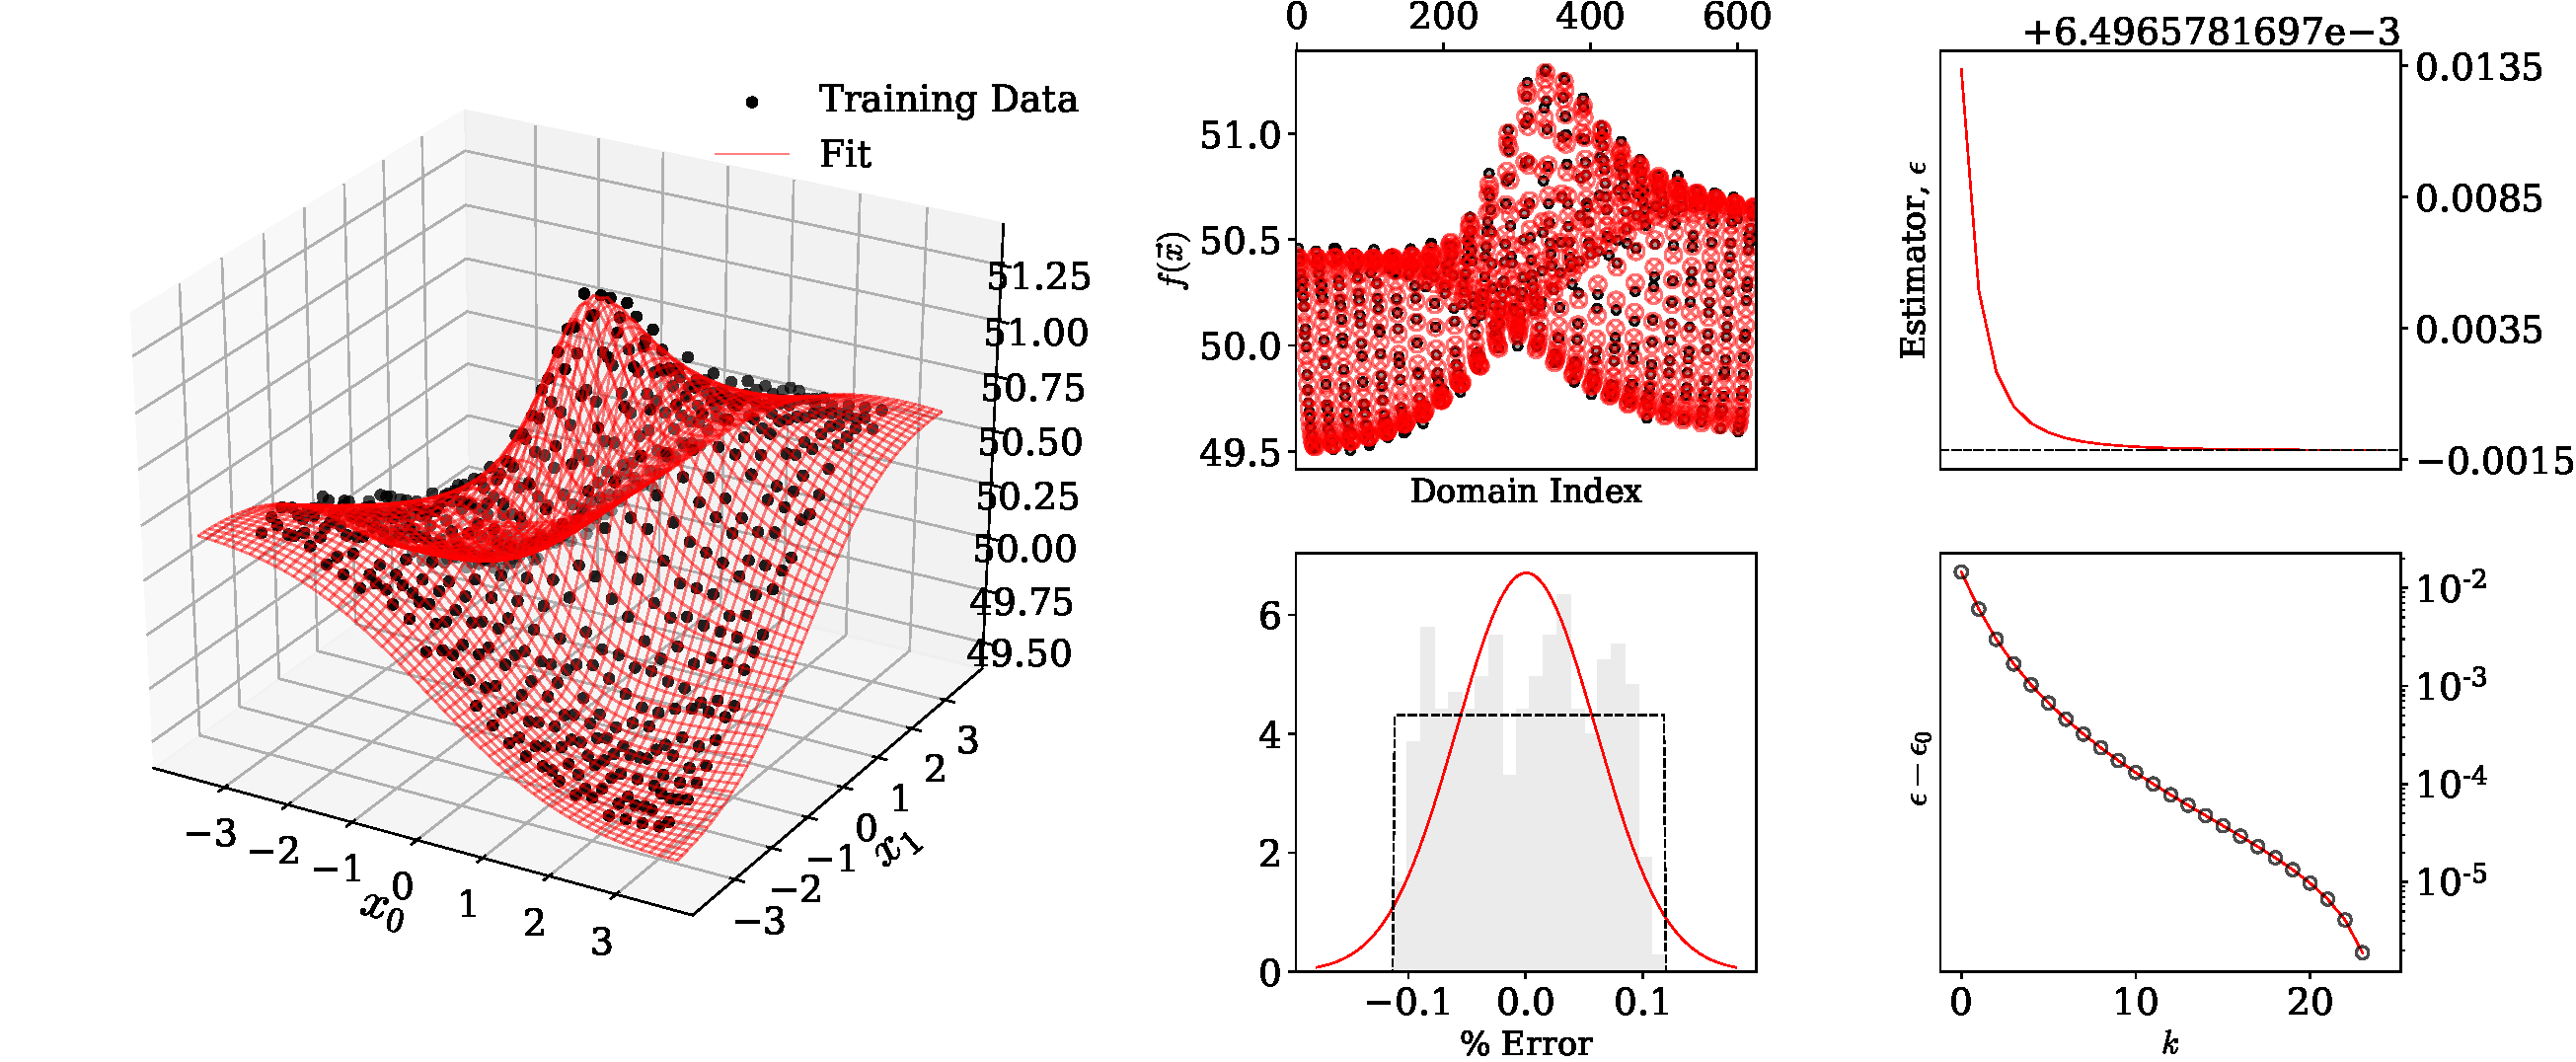
\includegraphics[width=\textwidth]{fig/issue3_summary.pdf}
  %
	\caption{ Standard summary plot for \gmvr. }
  %
  \label{fig:gmvrtoy}
  %
\end{figure*}


%
\begin{figure}[htb]
  %
  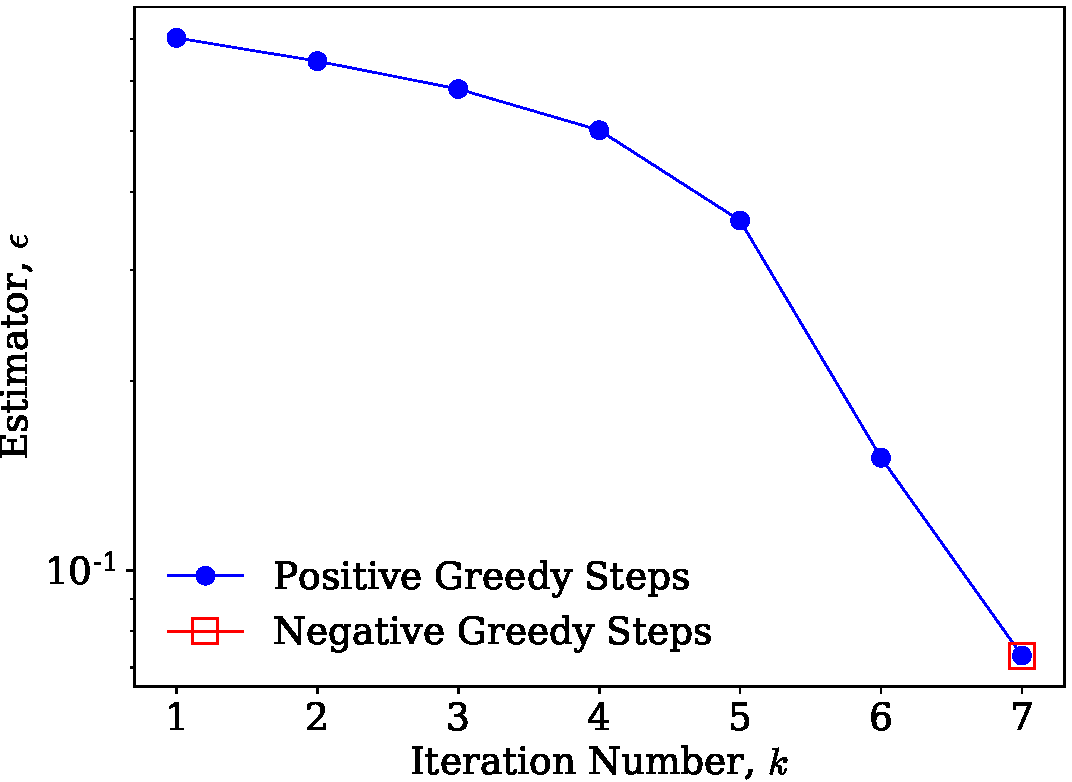
\includegraphics[width=0.45\textwidth]{fig/issue3_pgreedy.pdf}
	\caption{ Convergence of greedy process for \gmvr{} toy problem. }
  %
\end{figure}

%
\subsection{Modeling \qnm{} frequencies using \gmvp{}}
%
In seeking to apply \gmvp{} to select \qnm{} frequencies, we wish to impose a zero-damping constraint, namely that some frequencies are real as $\jf \rightarrow 1$.
%
We also wish the impose a domain transformation, $\kappa(\jf)$, such that $0 \leq \kappa \leq 1$ and the individual \qnm{} frequencies are morphologically simplified.
%
\par For the domain transformation, inspection of \qnm{} frequencies with $\ell \leq 5$ suggest that
%
\begin{align}
  \kappa(\jf) = \left( \ln( 2 - \jf ) / \ln(3) \right)^{1/(2-\ell+|m|)}
\end{align}
%
appropriately linearizes the sharp behavior of each frequency near $\jf=1$.
%
\par For the zero-damping constraint, when considering a \qnm{} frequency $\cw_{\lmn}$, zero-damping at $\jf=1$ implies that $\cw_{\lmn}(\kappa \approx 0)-m/2 \propto \kappa$, where $m/2$ is the well known limiting value for each \qnm{} frequencies real part as $\jf\rightarrow 1$.
%
% Plots of QNM frequencies
\begin{figure*}
  %
  \begin{tabular}{lcr}
    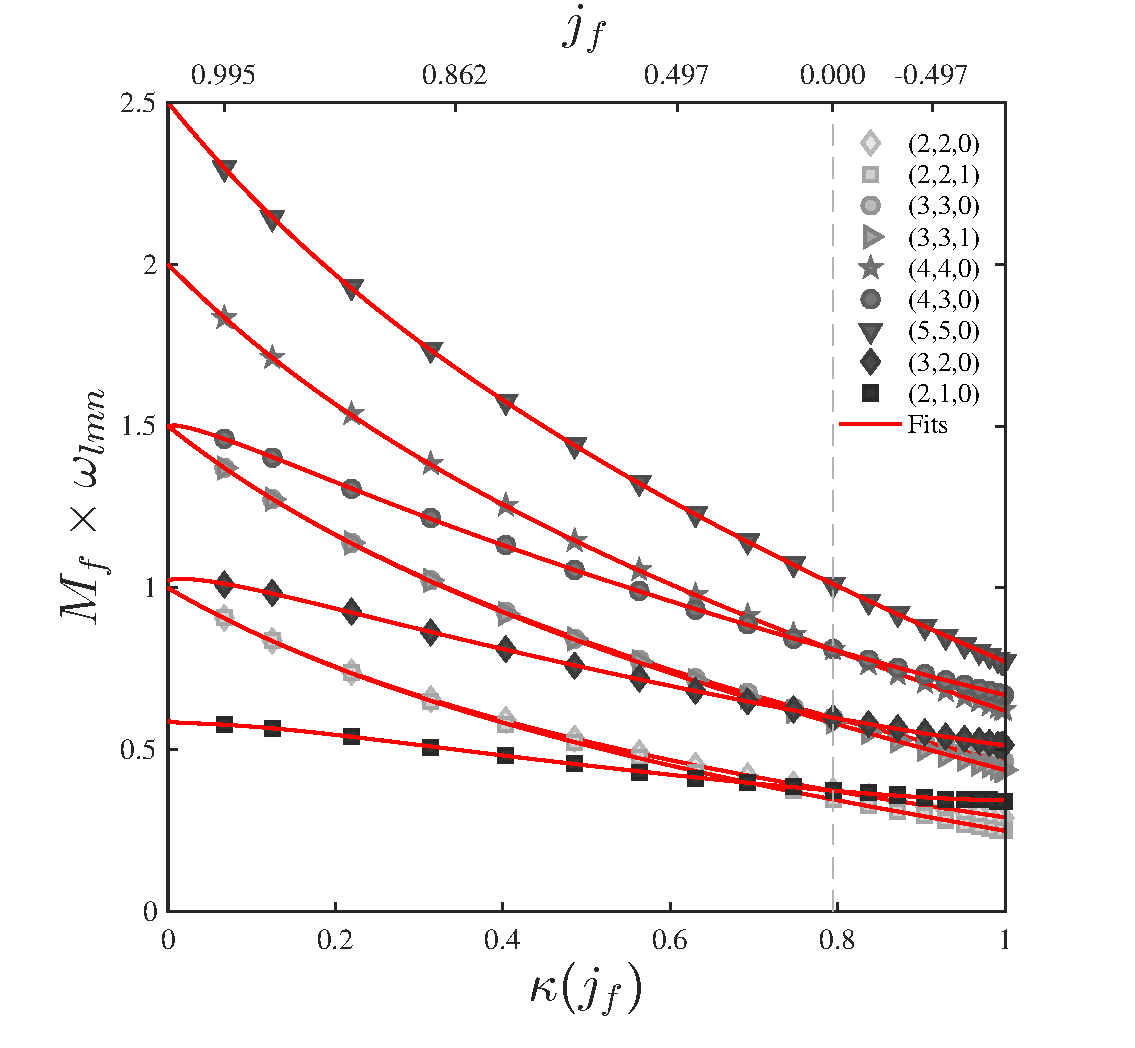
\includegraphics[width=\figfactor\textwidth]{fig/fits_w.pdf} & 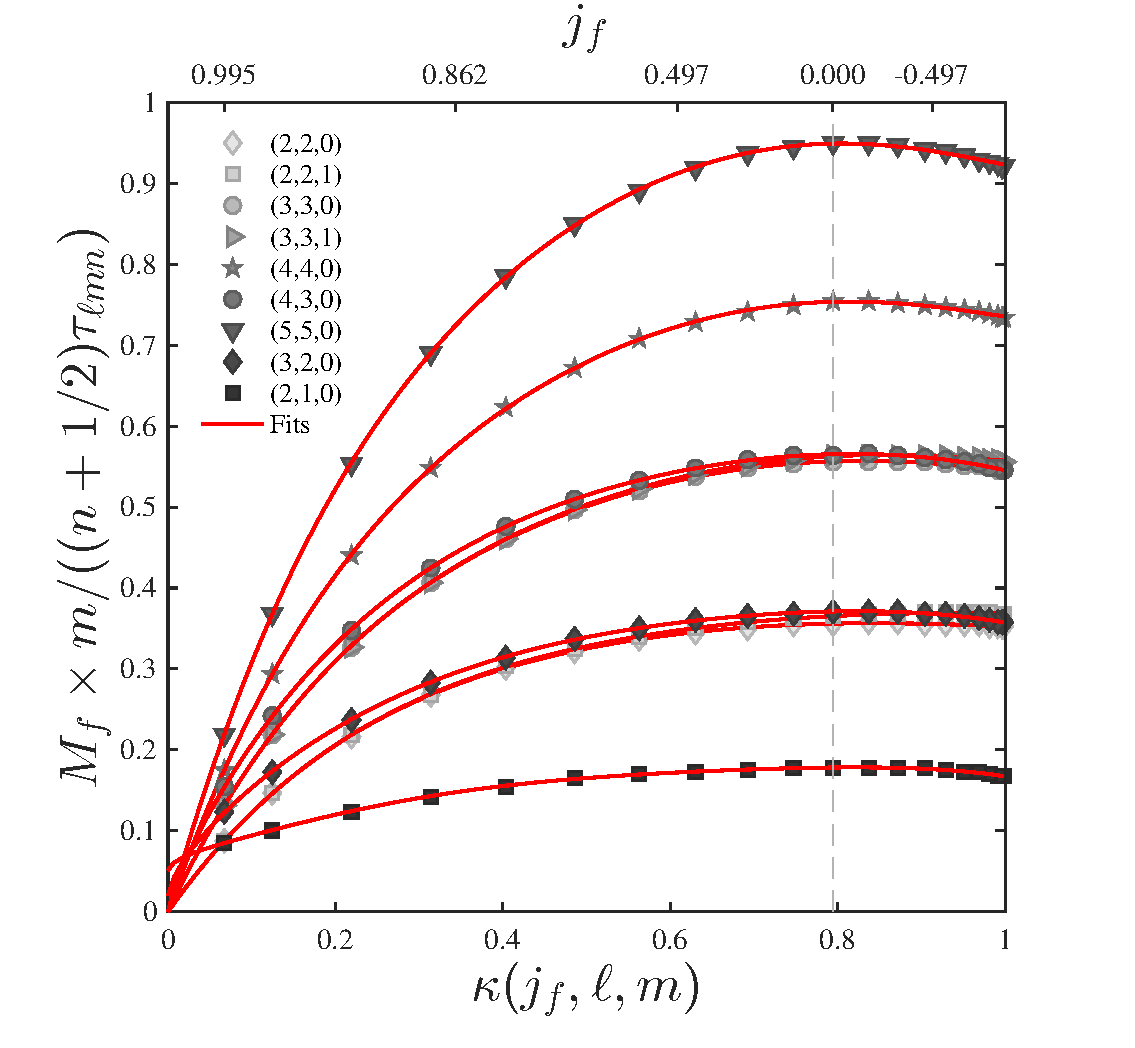
\includegraphics[width=\figfactor\textwidth]{fig/fits_tau.pdf}
  \end{tabular}
  %
	\caption{ Fits of dimensionless \qnm{} central frequencies (solid lines) along with select numerical values (grey markers) computed using Leaver's method \cite{Leaver85}.
  %
  Before the application of $\kappa(\j{})$, points are spaced between -\CwFitCalibrationRegion and \CwFitCalibrationRegion according to \CwFitCalibrationRegion times the $\sin$ of a fiducial angle which is uniformly spaced between $-\pi/2$ and $\pi/2$. Values of $\j{}$ are shown in the upper axis for $\kappa$ at $l=m$.
  %
  The grey dashed line marks the value of $\kappa$ where $\j{}=0$. Fits of dimensionless \qnm{} decay rates (solid lines) along with select numerical values (grey markers) computed using Leaver's method \cite{Leaver85}. }
  %
  \label{fig:qnms}
  %
\end{figure*}
%
% Plots of QNM frequencies
\begin{figure*}
  %
  \begin{tabular}{lcr}
    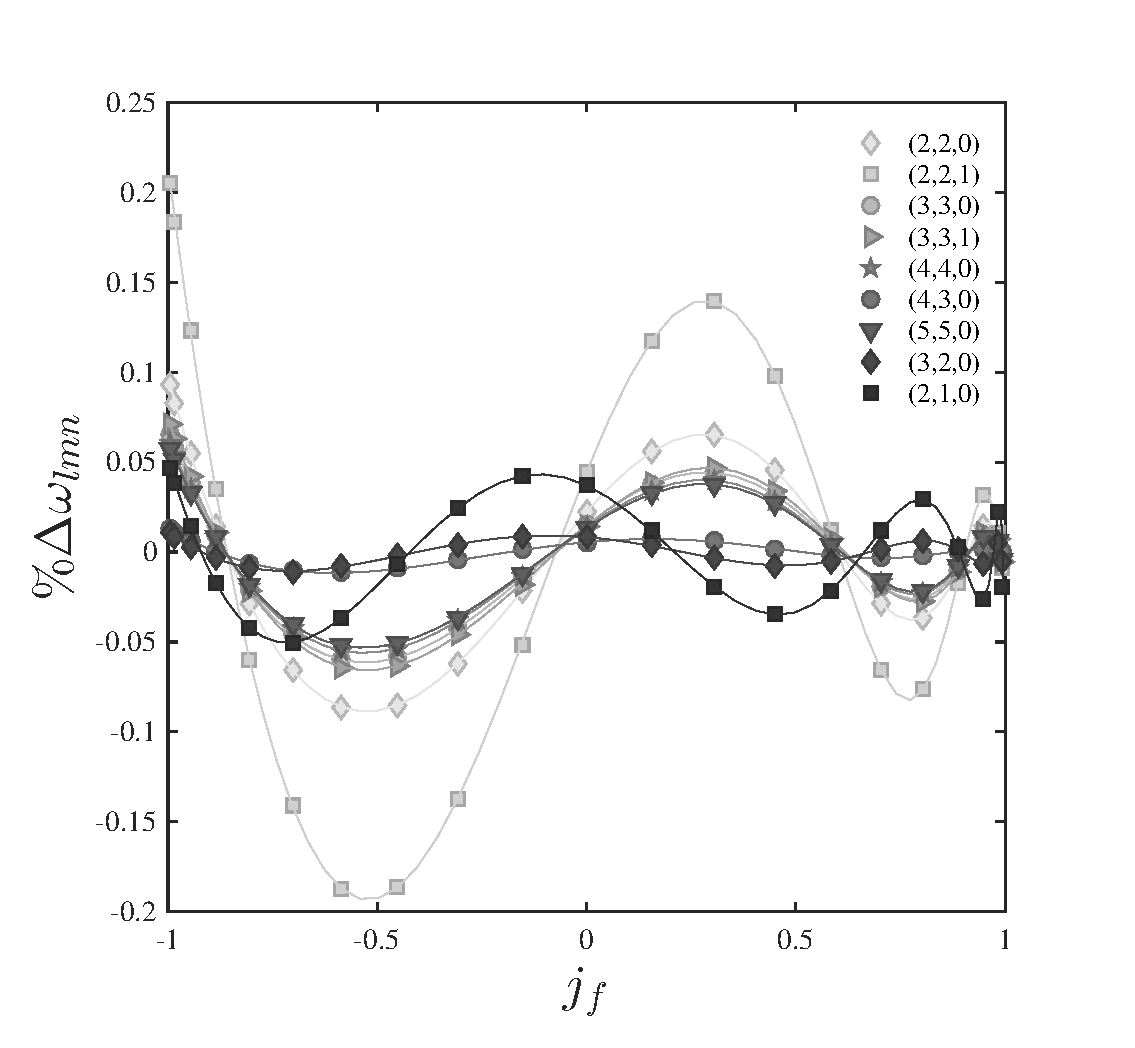
\includegraphics[width=\figfactor\textwidth]{fig/res_w.pdf} & 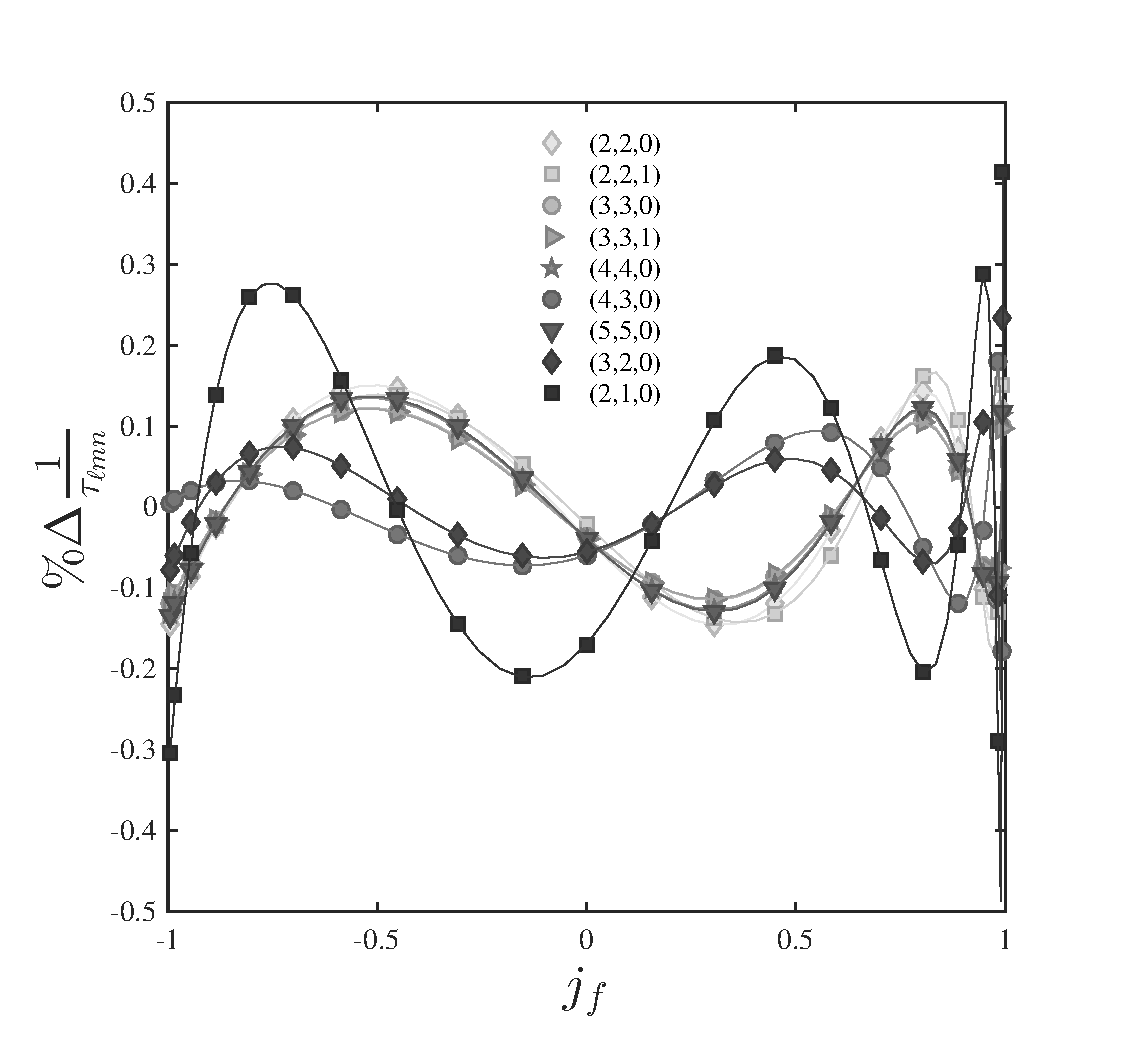
\includegraphics[width=\figfactor\textwidth]{fig/res_tau.pdf}
  \end{tabular}
  %
	\caption{ Fractional residual errors for fits of dimensionless \qnm{} central frequencies and decay times (solid lines) along with select numerical values (grey markers) computed using Leaver's method \cite{Leaver85}. }
  %
  \label{fig:qnm_err}
  %
\end{figure*}
%
This implies that
%
\begin{align}
  \label{eq:zd}
  \cw_{\lmn} = m/2 + \kappa \sum_{j=1}^{J} c_j \kappa^k \; .
\end{align}
%
In the case of the non-zero damped \qnm{s}, (e.g. $(\ell,m)=(3,2)$), a more general polynomial form may be adopted, namely,
%
\begin{align}
  \label{eq:nzd}
  \cw_{\lmn} = \sum_{j=0}^{J} c_j \kappa^k \; .
\end{align}
%
\par The polynomial content of \eqn{eq:zd} and \eqn{eq:nzd} is determined by \gmvp{}.
%
\eqns{eq:cw_fit_1}{eq:cw_fit_9} display the resulting polynomial models.
%
Although each model's fractional error is within 2\%, each is error is dominated by well known nonlinear oscillations which are considered to be outside of the experimental accuracy of current \gw{} efforts.
%
\par \fig{fig:qnms} displays select training points, as well as model fits for $\cw_{lmn}$'s real and imaginary parts.
%
For the right and left panels, simple polynomial behavior of each curve is a result of the displayed linear domain in $\kappa(\jf)$.
%
In the left panel, we have scaled $1/\tau_{\lmn}$ by factors for $m/(n+1/2)$ to place the \qnm{s} with $n=0$ and $n=1$ at approximately the same scale.
%
% Equations for QNM frequency fits
\begin{widetext}
	\begin{align}
	\label{eq:cw_fit_1}
	\cw_{220}(\kappa) \; &= \;\, 1.0 \, + \, \kappa \, (1.5578 e^{2.9031 i}\, + \, 1.9510  e^{5.9210 i} \kappa\, + \, 2.0997  e^{2.7606 i} \kappa ^ 2\, + \, 1.4109  e^{5.9143 i} \kappa ^ 3\, + \, 0.4106  e^{2.7952 i} \kappa ^ 4 \, )  \\
	\label{eq:cw_fit_2}
	\cw_{221}(\kappa) \; &= \;\, 1.0 \, + \, \kappa \, (1.8709 e^{2.5112 i}\, + \, 2.7192  e^{5.4250 i} \kappa\, + \, 3.0565  e^{2.2857 i} \kappa ^ 2\, + \, 2.0531  e^{5.4862 i} \kappa ^ 3\, + \, 0.5955  e^{2.4225 i} \kappa ^ 4 \, )  \\
	\label{eq:cw_fit_3}
	\cw_{330}(\kappa) \; &= \;\, 1.5 \, + \, \kappa \, (2.0957 e^{2.9650 i}\, + \, 2.4696  e^{5.9967 i} \kappa\, + \, 2.6655  e^{2.8176 i} \kappa ^ 2\, + \, 1.7584  e^{5.9327 i} \kappa ^ 3\, + \, 0.4991  e^{2.7817 i} \kappa ^ 4 \, )  \\ 
	\label{eq:cw_fit_4}
	\cw_{331}(\kappa) \; &= \;\, 1.5 \, + \, \kappa \, (2.3391 e^{2.6497 i}\, + \, 3.1399  e^{5.5525 i} \kappa\, + \, 3.5916  e^{2.3472 i} \kappa ^ 2\, + \, 2.4490  e^{5.4435 i} \kappa ^ 3\, + \, 0.7004  e^{2.2830 i} \kappa ^ 4 \, )  \\
	\label{eq:cw_fit_5}
	\cw_{440}(\kappa) \; &= \;\, 2.0 \, + \, \kappa \, (2.6589 e^{3.0028 i}\, + \, 2.9783  e^{6.0510 i} \kappa\, + \, 3.2184  e^{2.8775 i} \kappa ^ 2\, + \, 2.1276  e^{5.9897 i} \kappa ^ 3\, + \, 0.6034  e^{2.8300 i} \kappa ^ 4 \, )  \\
	\label{eq:cw_fit_6}
	\cw_{430}(\kappa) \; &= \;\, 1.5 \, + \, \kappa \, (0.2050 e^{0.5953 i}\, + \, 3.1033  e^{3.0162 i} \kappa\, + \, 4.2361  e^{6.0388 i} \kappa ^ 2\, + \, 3.0289  e^{2.8262 i} \kappa ^ 3\, + \, 0.9084  e^{5.9152 i} \kappa ^ 4 \, )  \\
	\label{eq:cw_fit_7}
	\cw_{550}(\kappa) \; &= \;\, 2.5 \, + \, \kappa \, (3.2405 e^{3.0279 i}\, + \, 3.4906  e^{6.0888 i} \kappa\, + \, 3.7470  e^{2.9212 i} \kappa ^ 2\, + \, 2.4725  e^{6.0365 i} \kappa ^ 3\, + \, 0.6994  e^{2.8766 i} \kappa ^ 4 \, )  \\
	\label{eq:cw_fit_8}
	\cw_{320}(\kappa) \; &= \;\,1.0225 e^{0.0049 i}\, + \, 0.2473  e^{0.6653 i} \kappa\, + \, 1.7047  e^{3.1383 i} \kappa ^ 2\, + \, 0.9460  e^{0.1632 i} \kappa ^ 3\, + \, 1.5319  e^{5.7036 i} \kappa ^ 4\\ \nonumber
	&\hspace{255pt}\, + \, 2.2805  e^{2.6852 i} \kappa ^ 5\, + \, 0.9215  e^{5.8417 i} \kappa ^ 6 \\
	\label{eq:cw_fit_9}
	\cw_{210}(\kappa) \; &= \;\,0.5891 e^{0.0435 i}\, + \, 0.1890  e^{2.2899 i} \kappa\, + \, 1.1501  e^{5.8101 i} \kappa ^ 2\, + \, 6.0459  e^{2.7420 i} \kappa ^ 3\, + \, 11.1263  e^{5.8441 i} \kappa ^ 4\\ \nonumber
	&\hspace{255pt}\, + \, 9.3471  e^{2.6694 i} \kappa ^ 5\, + \, 3.0384  e^{5.7915 i} \kappa ^ 6
\end{align}

\end{widetext}
%
%
\subsection{Modeling spherical-spheroidal inner-products using \gmvr{}}
%
%
% Equations for mixing coefficients
\begin{widetext}
  \begin{align}
   % (2, 2, 2, 2, 0)
  \label{eq:ys22220}
  \sigma_{22220} \, &= \, 0.99733\,e^{6.2813i} \, + 0.0075336 \, \frac{ 1.9624\,e^{3.0113i} \, + \, 14.592\,e^{5.0601i}\,\kappa \, + \, 28.761\,e^{1.629i}\,{\kappa}^{2} \, + \, 14.511\,e^{4.6362i}\,{\kappa}^{3} }{ 1 \, + \,   0.88674\,e^{3.0787i}\,\kappa \, + \, 1.002\,e^{0.13211i}\,{\kappa}^{2} \, + \, 0.082148\,e^{5.6369i}\,{\kappa}^{3} }   \\
   % (2, 1, 2, 1, 0)
  \label{eq:ys21210}
  \sigma_{21210} \, &= \, 0.99716\,e^{6.2815i} \, + 0.0063542 \, \frac{ 6026.9\,e^{1.8881i}  \, + \, 1.4345\times 10^5\,e^{4.5061i}\,\kappa \, + \, 3.5469\times 10^5\,e^{1.7327i}\,{\kappa}^{2} \, + \, 2.4038\times 10^5\,e^{5.1629i}\,{\kappa}^{3} }{ 1 \, + \,   73780\,e^{4.5545i}\,\kappa \, + \, 97494\,e^{1.398i}\,{\kappa}^{2} \, + \, 34815\,e^{4.5623i}\,{\kappa}^{3} }   \\
   % (2, 2, 2, 2, 1)
  \label{eq:ys22221}
  \sigma_{22221} \, &= \, 0.99683\,e^{6.2782i} \, + 0.020758 \, \frac{  0.71897\,e^{2.8084i}  \, + \,  15.077\,e^{4.8323i}\,\kappa \, + \, 31.139\,e^{1.585i}\,{\kappa}^{2} \, + \, 15.449\,e^{4.6727i}\,{\kappa}^{3} }{ 1 \, + \,   0.80592\,e^{3.3995i}\,\kappa \, + \, 0.69502\,e^{0.54275i}\,{\kappa}^{2} \, + \, 0.35613\,e^{5.9545i}\,{\kappa}^{3} }   \\
   % (3, 2, 3, 2, 0)
  \label{eq:ys32320}
  \sigma_{32320} \, &= \, 0.99009\,e^{6.2804i} \, + 0.02369 \, \frac{  1935.5\,e^{4.668i} \, + \,  71893\,e^{1.2395i}\,\kappa \, + \, 1.7055\times 10^5\,e^{5.0371i}\,{\kappa}^{2} \, + \, 1.2947\times 10^5\,e^{2.359i}\,{\kappa}^{3} }{ 1 \, + \,   38206\,e^{1.2254i}\,\kappa \, + \, 35811\,e^{3.9618i}\,{\kappa}^{2} \, + \, 8378.3\,e^{0.11726i}\,{\kappa}^{3} }   \\
   % (3, 3, 3, 3, 1)
  \label{eq:ys33331}
  \sigma_{33331} \, &= \, 0.99478\,e^{6.2688i} \, + 0.040478 \, \frac{ 0.67724\,e^{2.5797i}  \, + \,   4.4113\,e^{1.2501i}\,\kappa \, + \, 11.588\,e^{0.27959i}\,{\kappa}^{2} \, + \, 17.322\,e^{3.7904i}\,{\kappa}^{3} }{ 1 \, + \,   3.8782\,e^{2.2864i}\,\kappa \, + \, 3.4913\,e^{5.6655i}\,{\kappa}^{2} \, + \, 1.0368\,e^{2.9082i}\,{\kappa}^{3} }   \\
   % (3, 2, 2, 2, 1)
  \label{eq:ys32221}
  \sigma_{32221} \, &= \, 0.02203\,e^{0.16452i} \, + 0.073233 \, \frac{ 2.4374\,e^{6.1959i}  \, + \,   24.932\,e^{1.0181i}\,\kappa \, + \, 30.197\,e^{4.4047i}\,{\kappa}^{2} \, + \, 11.274\,e^{2.981i}\,{\kappa}^{3} }{ 1 \, + \,   11.397\,e^{3.9953i}\,\kappa \, + \, 10.915\,e^{5.8025i}\,{\kappa}^{2} \, + \, 7.2196\,e^{1.8176i}\,{\kappa}^{3} }   \\
   % (3, 3, 3, 3, 0)
  \label{eq:ys33330}
  \sigma_{33330} \, &= \, 0.99569\,e^{6.2785i} \, + 0.014546 \, \frac{ 1.7113\,e^{2.9527i}  \, + \,  7.2112\,e^{0.62811i}\,\kappa \, + \, 6.5381\,e^{4.6216i}\,{\kappa}^{2} \, + \, 4.451\,e^{2.9228i}\,{\kappa}^{3} }{ 1 \, + \,   1.4974\,e^{1.6687i}\,\kappa \, + \, 1.5288\,e^{5.3885i}\,{\kappa}^{2} \, + \, 0.52114\,e^{2.5471i}\,{\kappa}^{3} }   \\
   % (3, 2, 2, 2, 0)
  \label{eq:ys32220}
  \sigma_{32220} \, &= \, 0.020598\,e^{0.04743i} \, + 0.06919 \, \frac{ 2.399\,e^{6.2767i}  \, + \,  2.7657\,e^{2.133i}\,\kappa \, + \, 3.9562\,e^{4.653i}\,{\kappa}^{2} \, + \, 2.3364\,e^{2.6444i}\,{\kappa}^{3} }{ 1 \, + \,   1.0595\,e^{4.7865i}\,\kappa \, + \, 0.91308\,e^{2.887i}\,{\kappa}^{2} \, + \, 0.69468\,e^{0.1912i}\,{\kappa}^{3} }   \\
   % (4, 3, 3, 3, 0)
  \label{eq:ys43330}
  \sigma_{43330} \, &= \, 0.028112\,e^{0.048488i} \, + 0.086383 \, \frac{  2.3603\,e^{6.2662i}  \, + \,  12.087\,e^{0.47221i}\,\kappa \, + \, 30.626\,e^{3.3281i}\,{\kappa}^{2} \, + \, 16.328\,e^{6.1785i}\,{\kappa}^{3} }{ 1 \, + \,   4.9638\,e^{3.5931i}\,\kappa \, + \, 6.2552\,e^{6.2001i}\,{\kappa}^{2} \, + \, 1.4538\,e^{2.5539i}\,{\kappa}^{3} }   \\
   % (4, 3, 4, 3, 0)
  \label{eq:ys43430}
  \sigma_{43430} \, &= \, 0.98735\,e^{6.2795i} \, + 0.033028 \, \frac{ 13844\,e^{4.5601i}  \, + \,  7.0084\times 10^5\,e^{1.1067i}\,\kappa \, + \, 1.843\times 10^6\,e^{4.8808i}\,{\kappa}^{2} \, + \, 1.4367\times 10^6\,e^{2.1412i}\,{\kappa}^{3} }{ 1 \, + \,   3.5667\times 10^5\,e^{1.0149i}\,\kappa \, + \, 3.274\times 10^5\,e^{3.7746i}\,{\kappa}^{2} \, + \, 88621\,e^{0.10095i}\,{\kappa}^{3} }   \\
   % (4, 4, 4, 4, 0)
  \label{eq:ys44440}
  \sigma_{44440} \, &= \, 0.99478\,e^{6.2776i} \, + 0.024791 \, \frac{ 1.2434\,e^{2.9616i}  \, + \,  6.5172\,e^{0.79835i}\,\kappa \, + \, 7.7748\,e^{4.2485i}\,{\kappa}^{2} \, + \, 1.1577\,e^{1.5905i}\,{\kappa}^{3} }{ 1 \, + \,   0.44548\,e^{1.2496i}\,\kappa \, + \, 0.59437\,e^{5.6732i}\,{\kappa}^{2} \, + \, 0.24743\,e^{2.8292i}\,{\kappa}^{3} }   \\
   % (5, 5, 5, 5, 0)
  \label{eq:ys55550}
  \sigma_{55550} \, &= \, 0.99434\,e^{6.2773i} \, + 0.03126 \, \frac{ 1.0904\,e^{2.9712i}  \, + \,  6.5508\,e^{0.93398i}\,\kappa \, + \, 8.0558\,e^{4.2881i}\,{\kappa}^{2} \, + \, 0.92971\,e^{1.0436i}\,{\kappa}^{3} }{ 1 \, + \,   0.23128\,e^{1.7666i}\,\kappa \, + \, 0.54958\,e^{5.9178i}\,{\kappa}^{2} \, + \, 0.213\,e^{3.0092i}\,{\kappa}^{3} }
\end{align}

\end{widetext}

% Plots of mixing coefficients
\begin{figure*}
  %
  \begin{tabular}{lcr}
    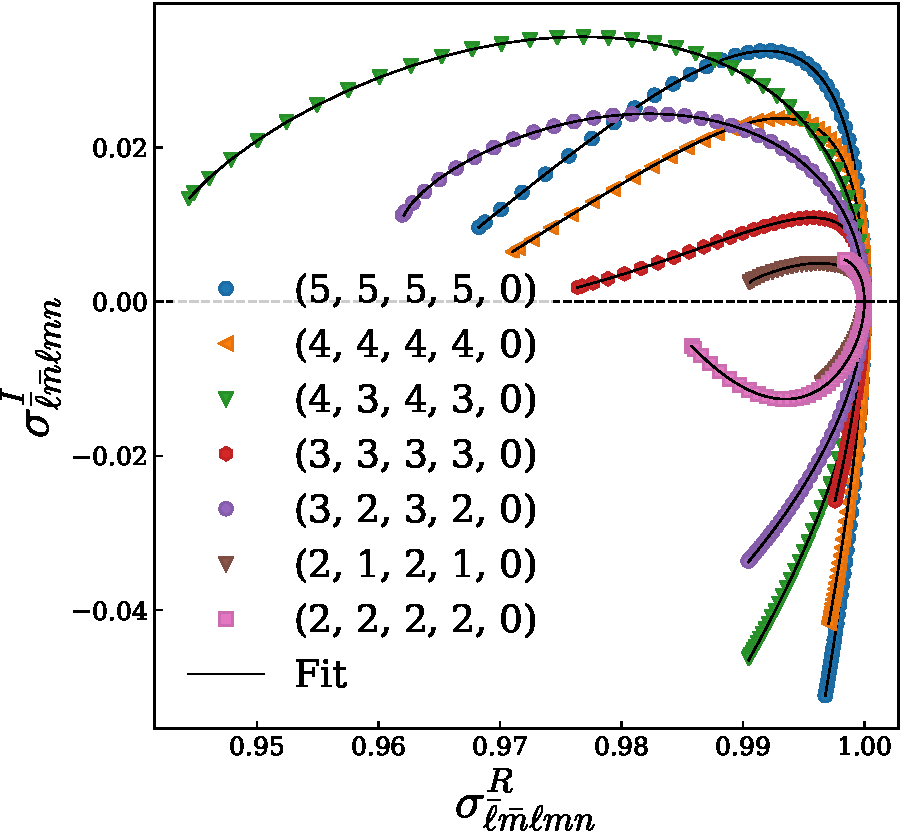
\includegraphics[width=\figfactor\textwidth]{fig/issue2_ysprod_1.pdf} & 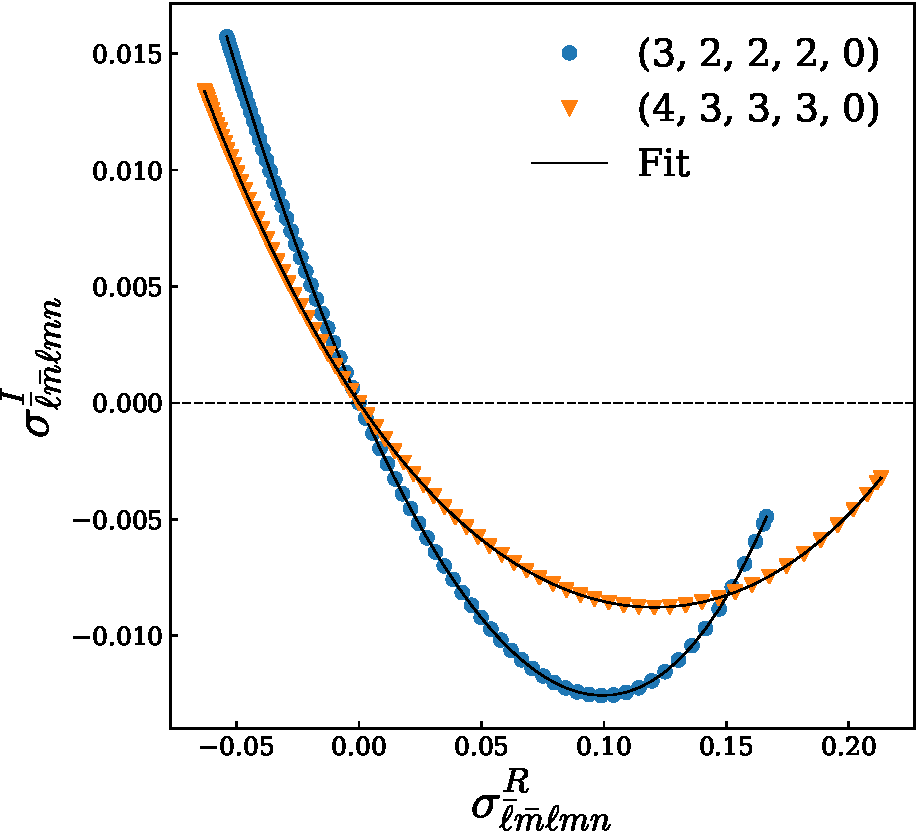
\includegraphics[width=\figfactor\textwidth]{fig/issue2_ysprod_2.pdf}
  \end{tabular}
  %
	\caption{ Spherical-spheroidal harmonic mixing coefficients. }
  %
\end{figure*}

% Plots of mixing coefficients
\begin{figure*}
  %
  \begin{tabular}{lcr}
    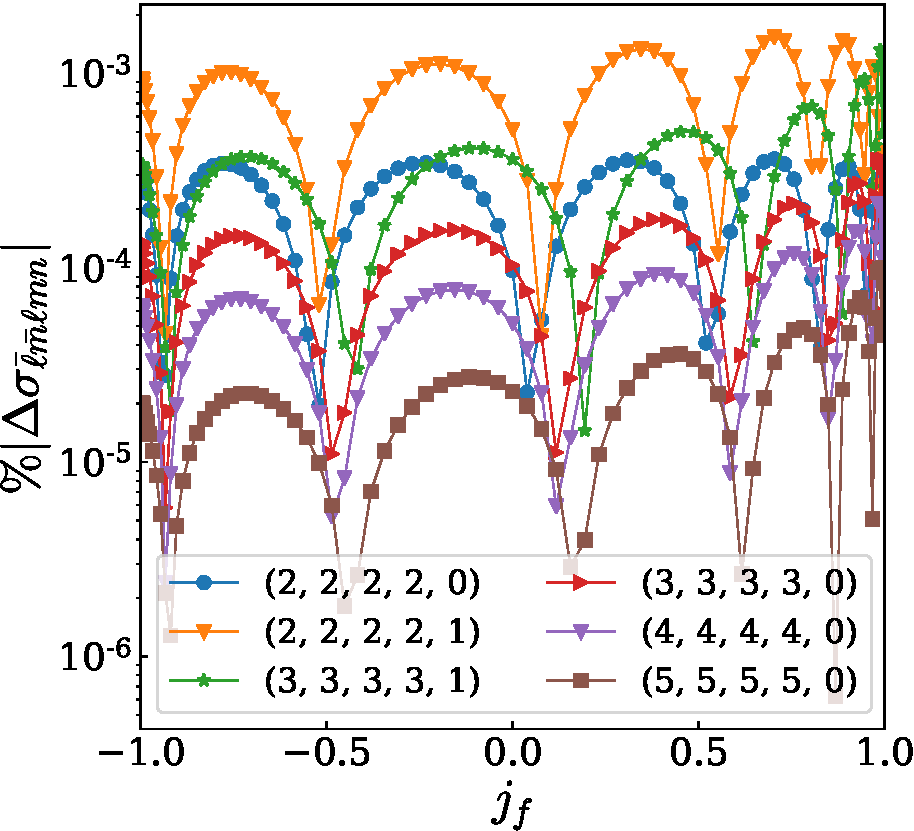
\includegraphics[width=\figfactor\textwidth]{fig/issue2_ysprod_3.pdf} & 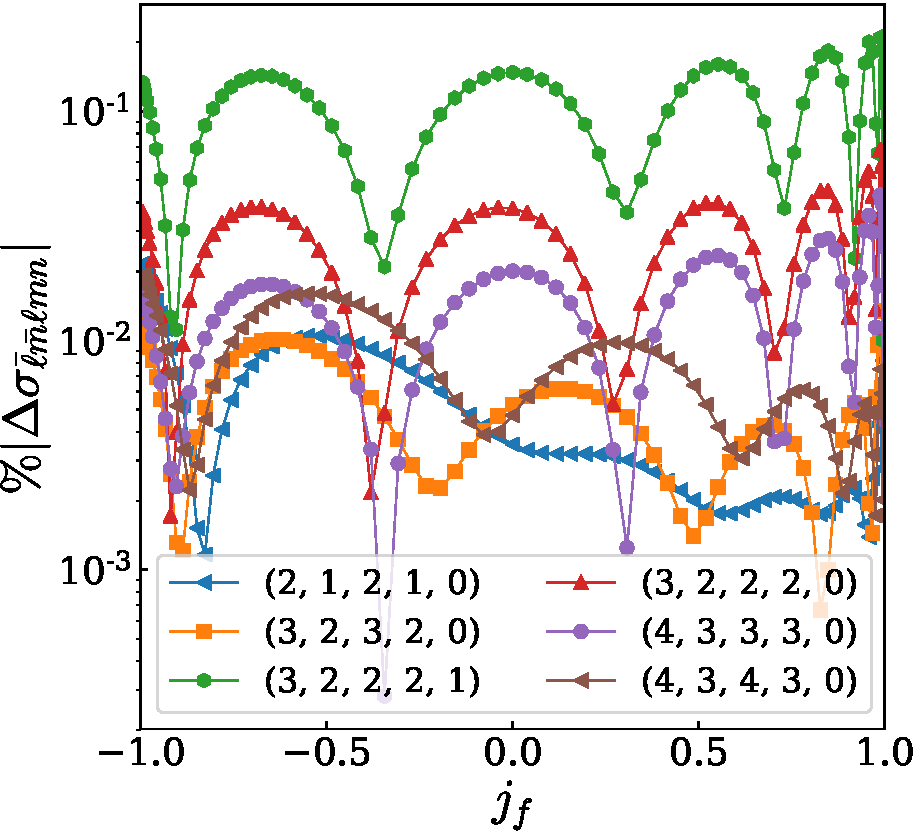
\includegraphics[width=\figfactor\textwidth]{fig/issue2_ysprod_4.pdf}
  \end{tabular}
  %
	\caption{ Percentage residual errors for spherical-spheroidal harmonic mixing coefficient models. }
  %
\end{figure*}



%
\section{Discussion}
\label{discuss}

% %%%%%%%%%%%%%%%%%%%%%%%%%%%%%%%%%%%%%%%%%%%%%%%%% %
\bibliographystyle{ieeetr}
\bibliography{src/mvf.bib}
\end{document}
